\section{Results and Discussion}

The scope of experiments in this project involve extensive use of AnACor, the prototype software used at beamline I23 for adding an analytical correction to reflections and reflection intensities \cite{Lu}. Previous work from I23 has documented the successes of tomographic reconstruction and segmentation pipelines to determine analytical absorption factors \cite{Kazantsev2021}; however, AnACor has only recently become the routine for this. The software is still in its developing stages with many reoccurring errors which limit our ability to do data processing and the reliability of results. Validation of the experimental results is therefore still necessary when possible.

One example of a step taken to improve reliability in this project is when samples containing solely the mother-liquor that crystals were grown in were available, tomography data would be collected on these as well as the crystal samples. The segmentation of loops containing only liquor allow for more reliable thresholds to be applied with fewer materials to account for, and therefore produces more accurate coefficients.

Since low-energy tomographic scans are prone to high contrast artefacts which limit visibility in the segmentation, tomography scans intended for diffraction experiments collected at or below 3 keV would be collected at 3.5 keV, in addition to the low energy. Distinguishing between materials in the 3.5 keV tomography scans is somewhat easier, and therefore provides better segmentation for the reflection data collected at lower energies.

%Finally ... preliminary tests

\subsection{Preliminary tests on AnACor}

Because the final reflection data heavily relies on the accuracy of absorption factors, the first experiments conducted for this project were a validation of the accuracy of AnACor's pre-process calculations. Theoretical absorption coefficients are given by the reciprocal of the attenuation length, which can be calculated for a material from its chemical formula, density, and the energy in question. The first experiment on AnACor used crystals of ethylene glycol and santovac to compare experimentally calculated coefficients from the software with theoretical coefficients.

The experimental coefficients of santovac, published in \cref{santovac_table}, are within 1.5 \% of the theoretical value for energies between 3 and 4.5 keV. This difference, however, appears to grow with energy, with a nearly 7\% difference at 6 keV. A similar trend is seen in \cref{ethylene_table} with the sudden jump from 1.2 \% at 5 keV to 6.3 \% at 6 keV for ethylene glycol.

Judging from the results of these two proteins alone, AnACor appears to overestimate coefficients at higher energies and similarly underestimates coefficients at lower energies. A possible explanation for the latter is the effect of high contrast at low energies limiting distinctions between materials; this however does not explain the overestimates at higher energies. It is also possible that the calculations do not sufficiently account for the changing dependence of absorption on wavelength, which is less strong at higher energies and would explain the the discrepancies.

A second validation experiment on AnACor involved samples of chlorite dismutase (Cld) and the membrane protein OmpK36 GD. Data on these two samples has already been analysed in Lu \textit{et al.} \cite{Lu} to compare the same approaches for absorption corrections discussed in this work: a \ac{sh} correction, analytical, and a combination of the two. The aim of this subsequent experiment, was to assess the accuracy of the absorption coefficients of crystal and liquor published in this paper. This was tested with the assumption that the accuracy would correlate to the best possible data quality, where the intensity to uncertainty ($I / \sigma$) peaks and the $R_{merge}$ factors are diminished.

Taking the coefficients published in this paper as a reference and varying both in intervals of \pm 10, sets up a variety of possible combinations of coefficient pairs which can together elucidate the optimal amount of variation in both for improving the merging statistics. The coefficients were varied from -20 \% to + 20 \%; after preliminary results were collected, the liquor coefficients were varied a further interval up to + 30 \%, giving a total of 30 possible coefficient variations. %The crystal reference was

The merging statics for all 30 AnACor experiments are shown in \cref{fig:cld_stats} for Cld and in \cref{fig:ompk_stats} for Ompk. The merging statistics of Cld tell a clearer story than that of Ompk: in \cref{fig:cld_stats} the $I/\sigma$ peaks between +10 and +20\% in the crystal factor, and +10\% for liquor; then looking at the R-factors, these values are minimised at the same variation. This indicates to the combination of coefficients that is presumably the most accurate for these materials, as it provides the best merging statistics.

While the differences in the maximum $I/\sigma$ and minimum R factors to their respective values at $\pm0,\pm0$ are small, in a perfect experiment these optimal statistics would align at $\pm0,\pm0$, as this would indicate that the references AnACor calculated are very good estimates. The underestimation here could be caused by several factors, including poor segmentation or insufficient threshold selections in pre-processing. Nonetheless, this procedure is still useful in correcting for small errors that deter AnACor from obtaining the true values. 

The Ompk results, shown in \cref{fig:ompk_stats}, are less clear by comparison. Despite the fact that there is an boundary where $I/\sigma$ is maximised, the R-factors do not change smoothly between experiments. Instead, there are only 3 values of the R-factor across all 30 runs with no incremental changes in between. This is a limitation in finding the optimal variation of coefficients, as the R-factor cannot be corroborated with the optimal $I/\sigma$.

%Establishing X-ray tomography as a valid approach: references for absorption correction calculations

%3D plots of finding the most optimal ACs for crystal and liquor using AnACor's AC values at 0.5 acceptance percentage as the reference

%This validation experiment ultimately took AC values calculated by AnACor in its pre-processing stage as a reference to run the post-processing of AnACor on a combination of AC of crystal and liquor varied in several increments from the reference. The aim of this was a check of AnACor's accuracy in determining the optimal AC that maximise the $I/ \sigma$ results while minimising the $R_{merge}$ factor.

In the interest of time, this validation check was not applied to the crystals investigated in the remainder of this project. Nonetheless, the experiment is a useful validation for finding the optimal absorption coefficients from AnACor for merging statistics. The scripts for this experiment have been complied to allow for users at I23 to apply this procedure to future tomography data. %A template of the scripts can be found at GitHub.


\subsection{Comparison of a spherical harmonics, analytical, and coupled approach} % empirical ?
% to absorption corrections
The primary focus of this project was to investigate the potential improvements in data quality by applying an analytical correction to diffraction data.
%Merging statistics and anomalous peak heights \cite{Lu}
In the interest of observing the effects of high absorption, crystal samples were largely collected at 3.0 and 3.5 keV, some of the lowest energies accessible to I23.

The first sample to be used for this investigation was a test crystal of thaumatin, collected at 3.0, 3.5, 4.0, and 4.5 keV. Because this early experiment was used primarily for segmentation practice, the results for the merging statistics can be found in the Appendix in \cref{fig:thaum1_stats}. Despite the segmentation being a rough model, the analytical approach already showed an improvement from \ac{sh}, with the two datasets at lower energies favouring \ac{acsh}, and the remaining datasets favouring \ac{aac}.

Subsequent tomography experiments were performed on two protein crystals of thermolysin. The first crystal, referred to as Thermolysin 1, was collected at three energies: 3.0, 3.5, and 3.8 keV, with datasets of varying orientations of $\kappa$ and $\phi$ at each energy, as listed in \cref{diffration_table}. The subsequent thermolysin crystal was collected only at 3.0 and 3.5 keV with the $\kappa$ and $\phi$ orientations also specified in \cref{diffration_table}.

\begin{figure}
    \centering
    \begin{tabular}{cc}
    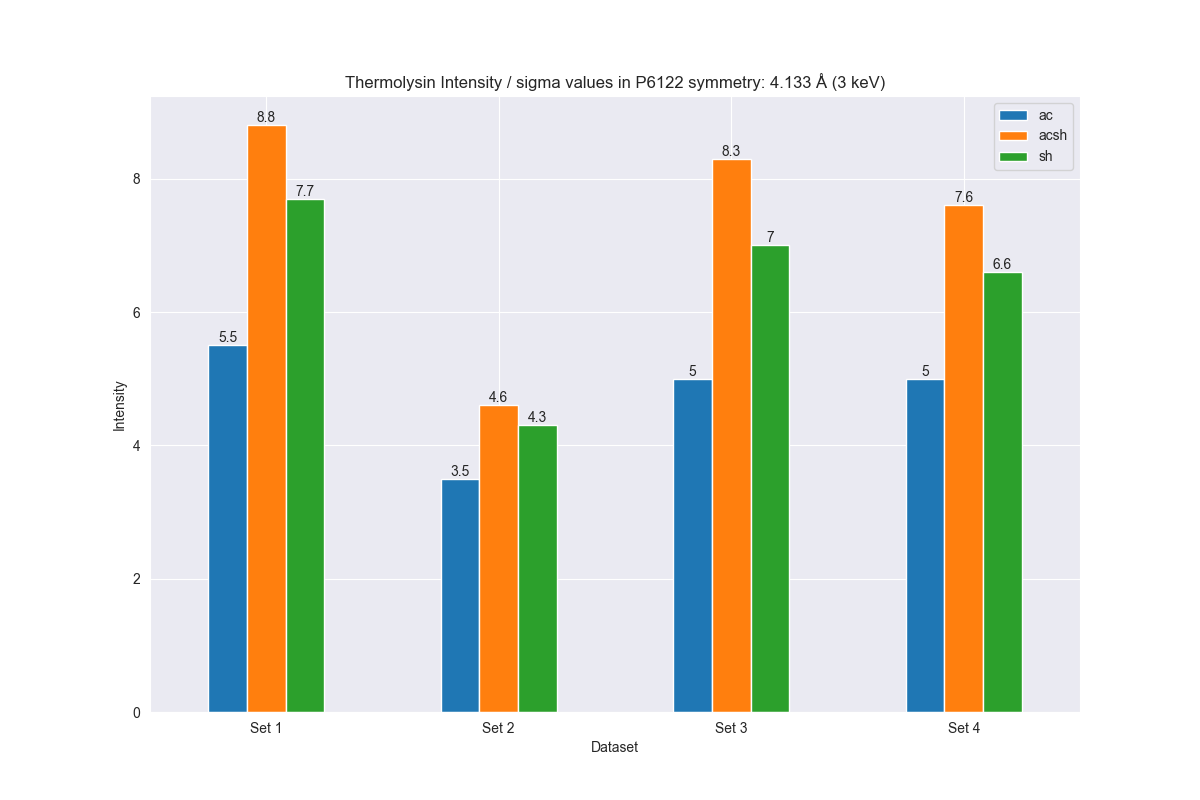
\includegraphics[width = 0.5\textwidth]{plots/exp1/tlys_9_P6122/3p0_I_over_sigma.png} & 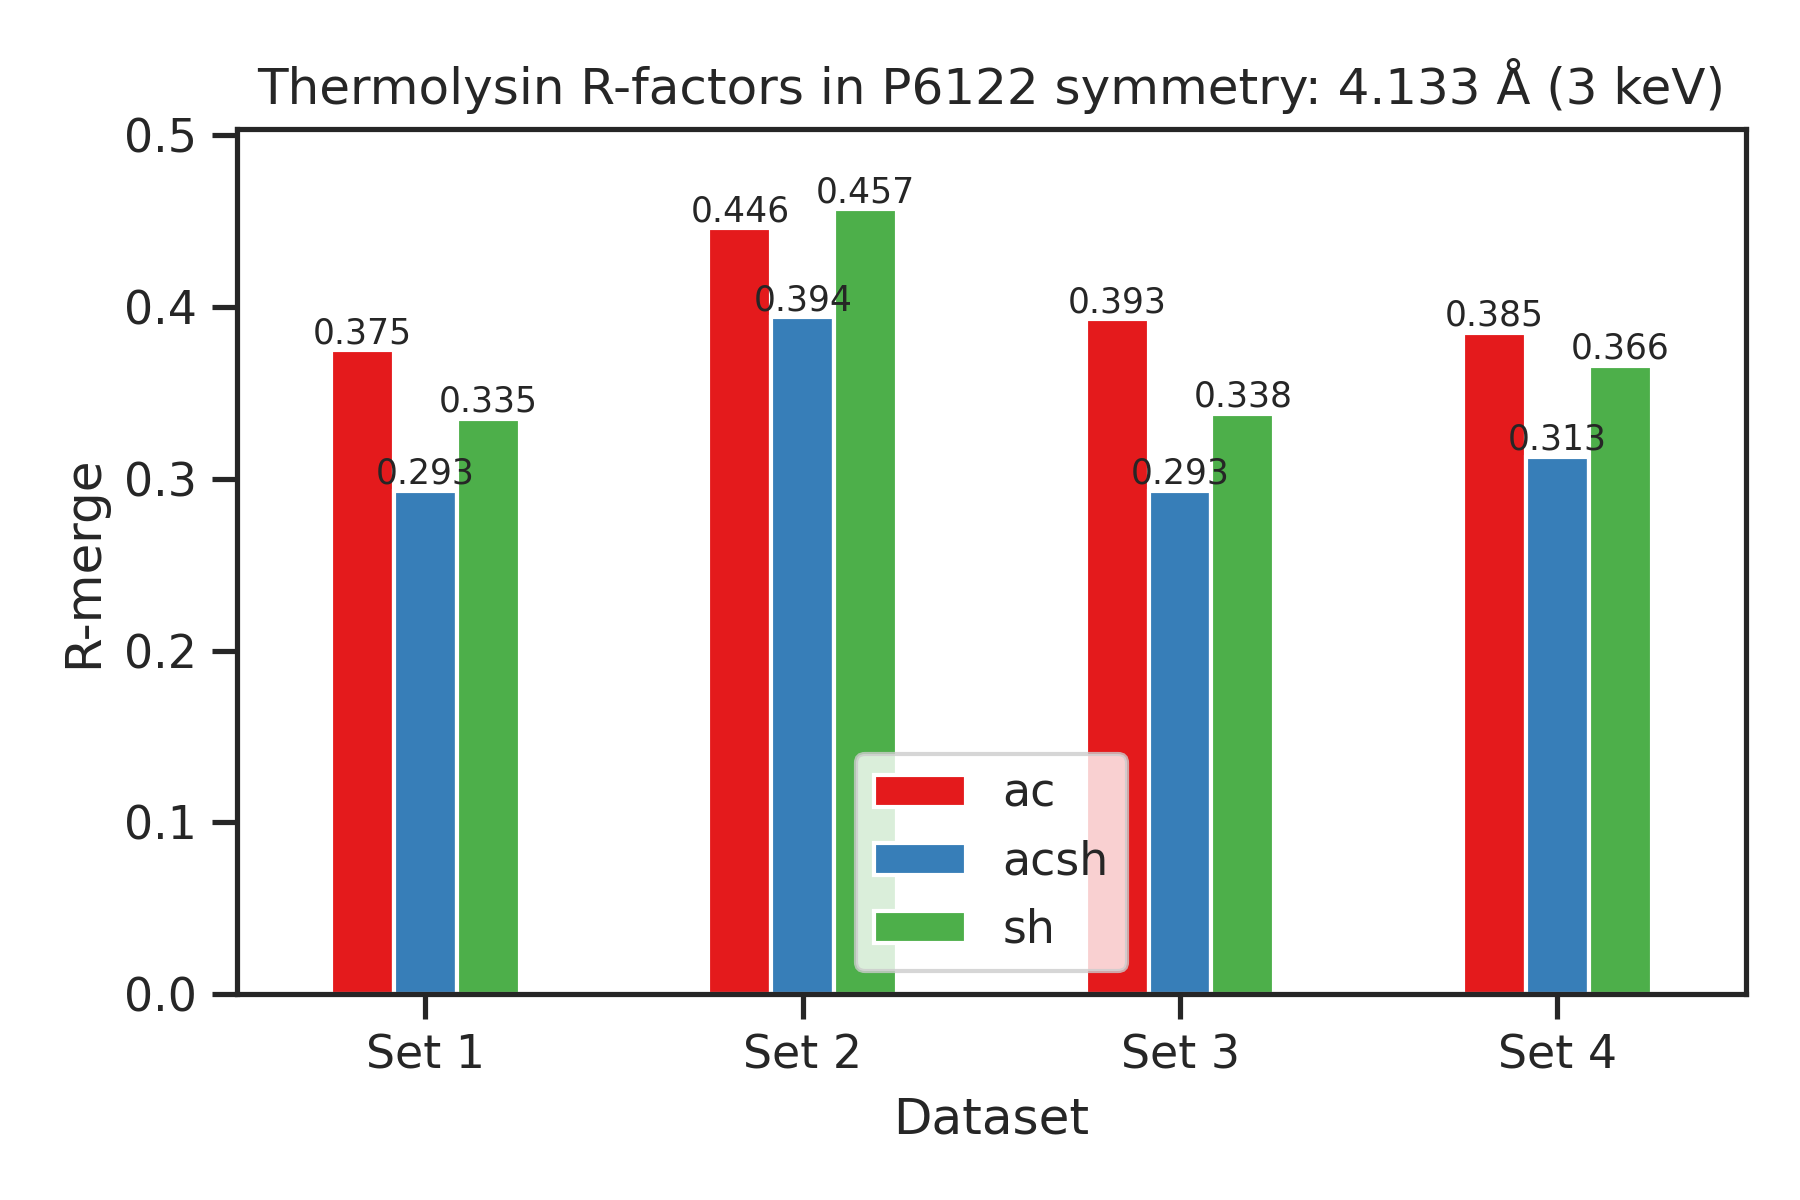
\includegraphics[width = 0.5\textwidth]{plots/exp1/tlys_9_P6122/3p0_rmerges.png}
    \end{tabular}
    \caption{Merging statistics for Thermolysin 1 at 3.0 keV.}
    \label{fig:tlys_9_3p0}
\end{figure}

\begin{figure}
    \centering
    \begin{tabular}{cc}
    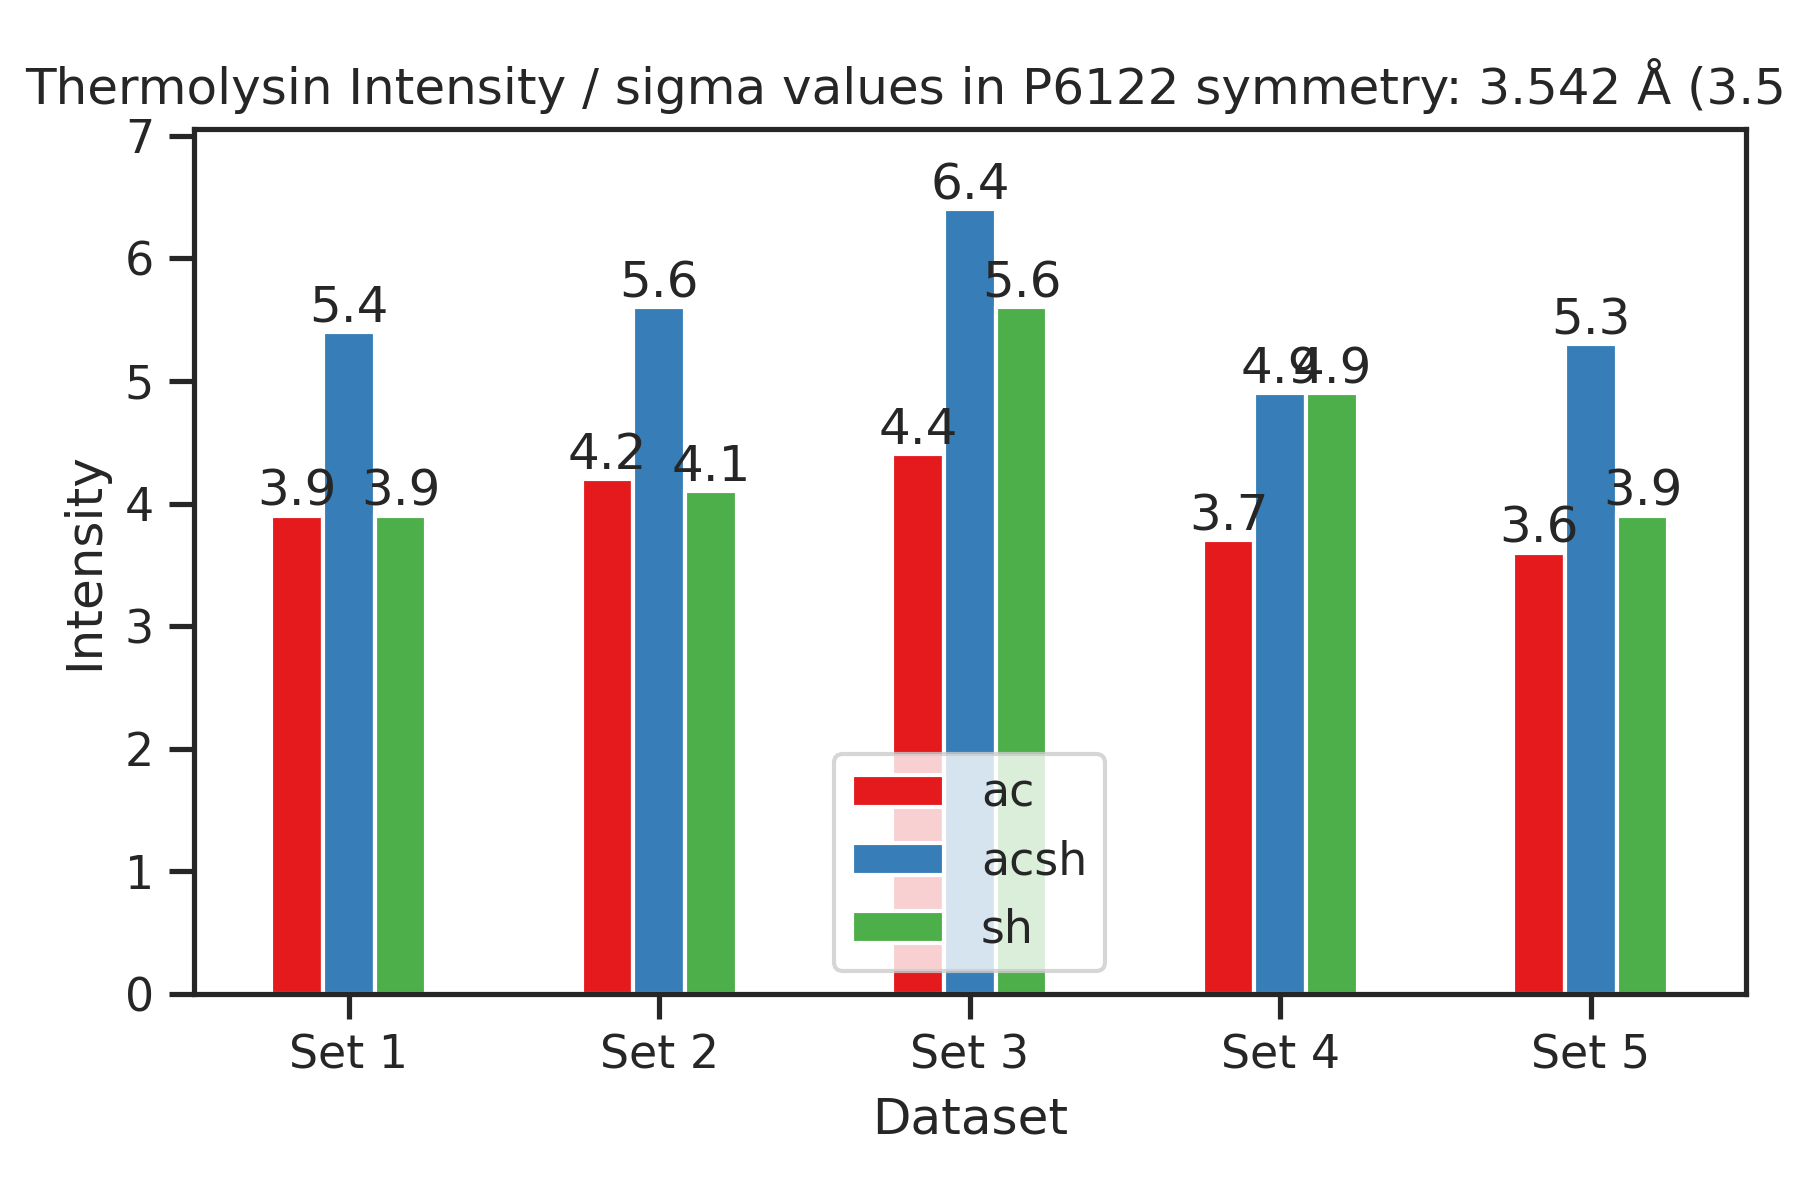
\includegraphics[width = 0.5\textwidth]{plots/exp1/tlys_9_P6122/3p5_I_over_sigma.png} & 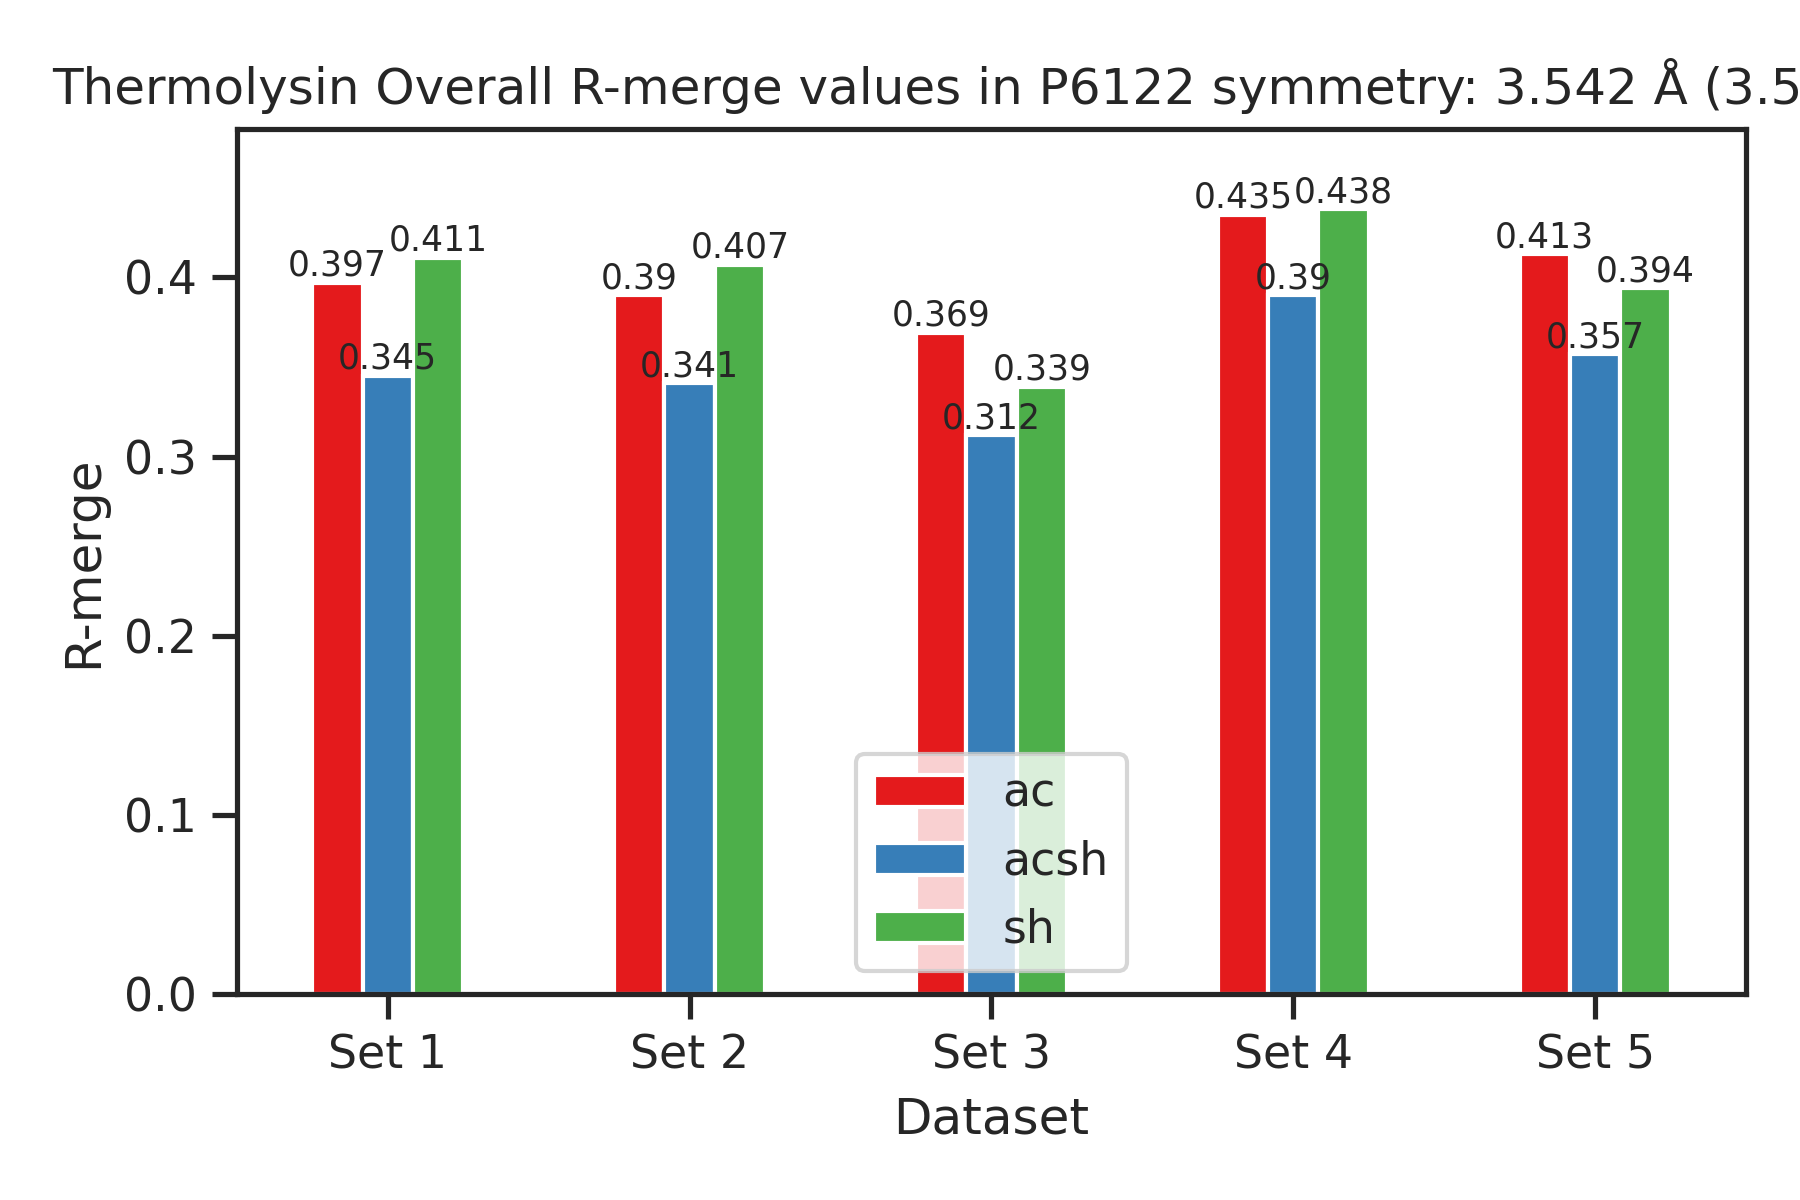
\includegraphics[width = 0.5\textwidth]{plots/exp1/tlys_9_P6122/3p5_rmerges.png}
    \end{tabular}
    \caption{Merging statistics for Thermolysin 1 at 3.5 keV.}
    \label{fig:tlys_9_3p5}
\end{figure}

\begin{figure}[h]
    \centering
    \begin{tabular}{cc}
    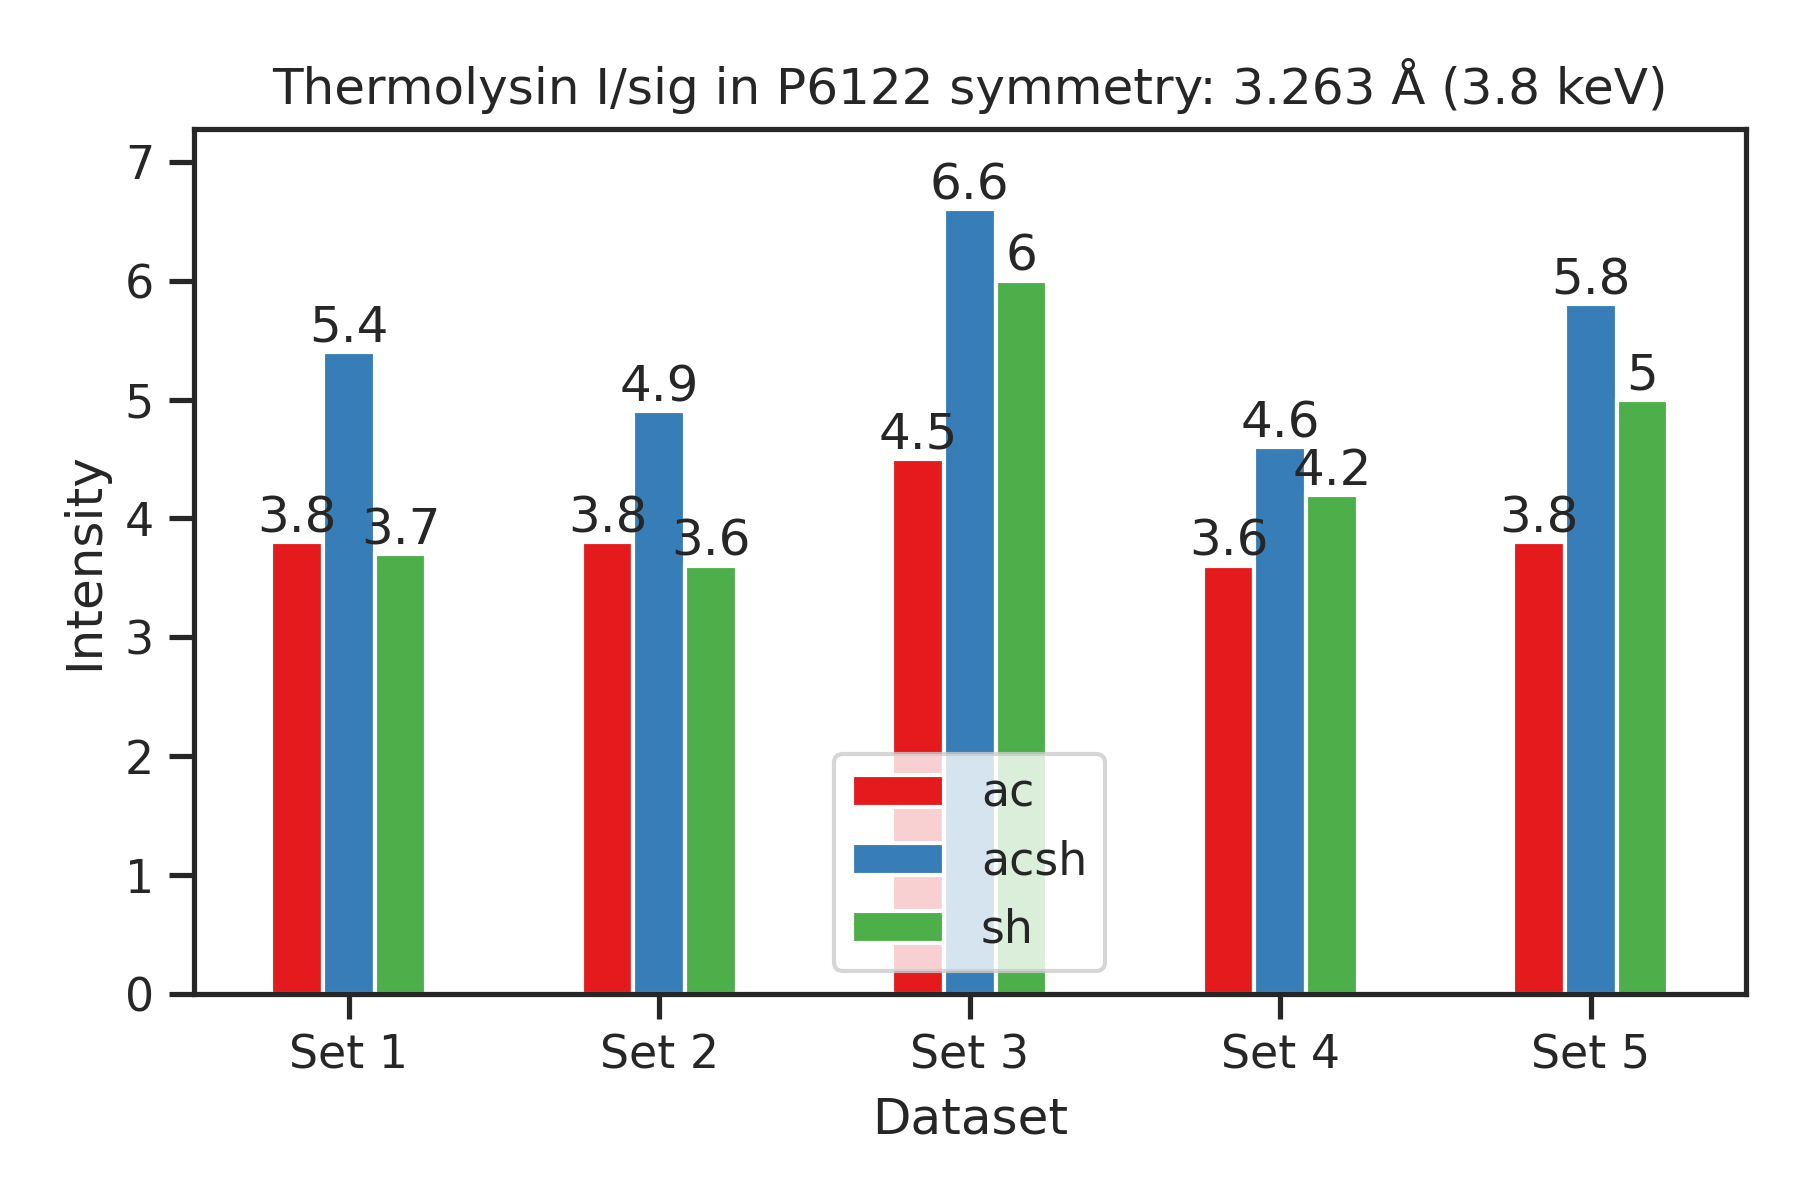
\includegraphics[width = 0.5\textwidth]{plots/exp1/tlys_9_P6122/3p8_I_over_sigma.png} & 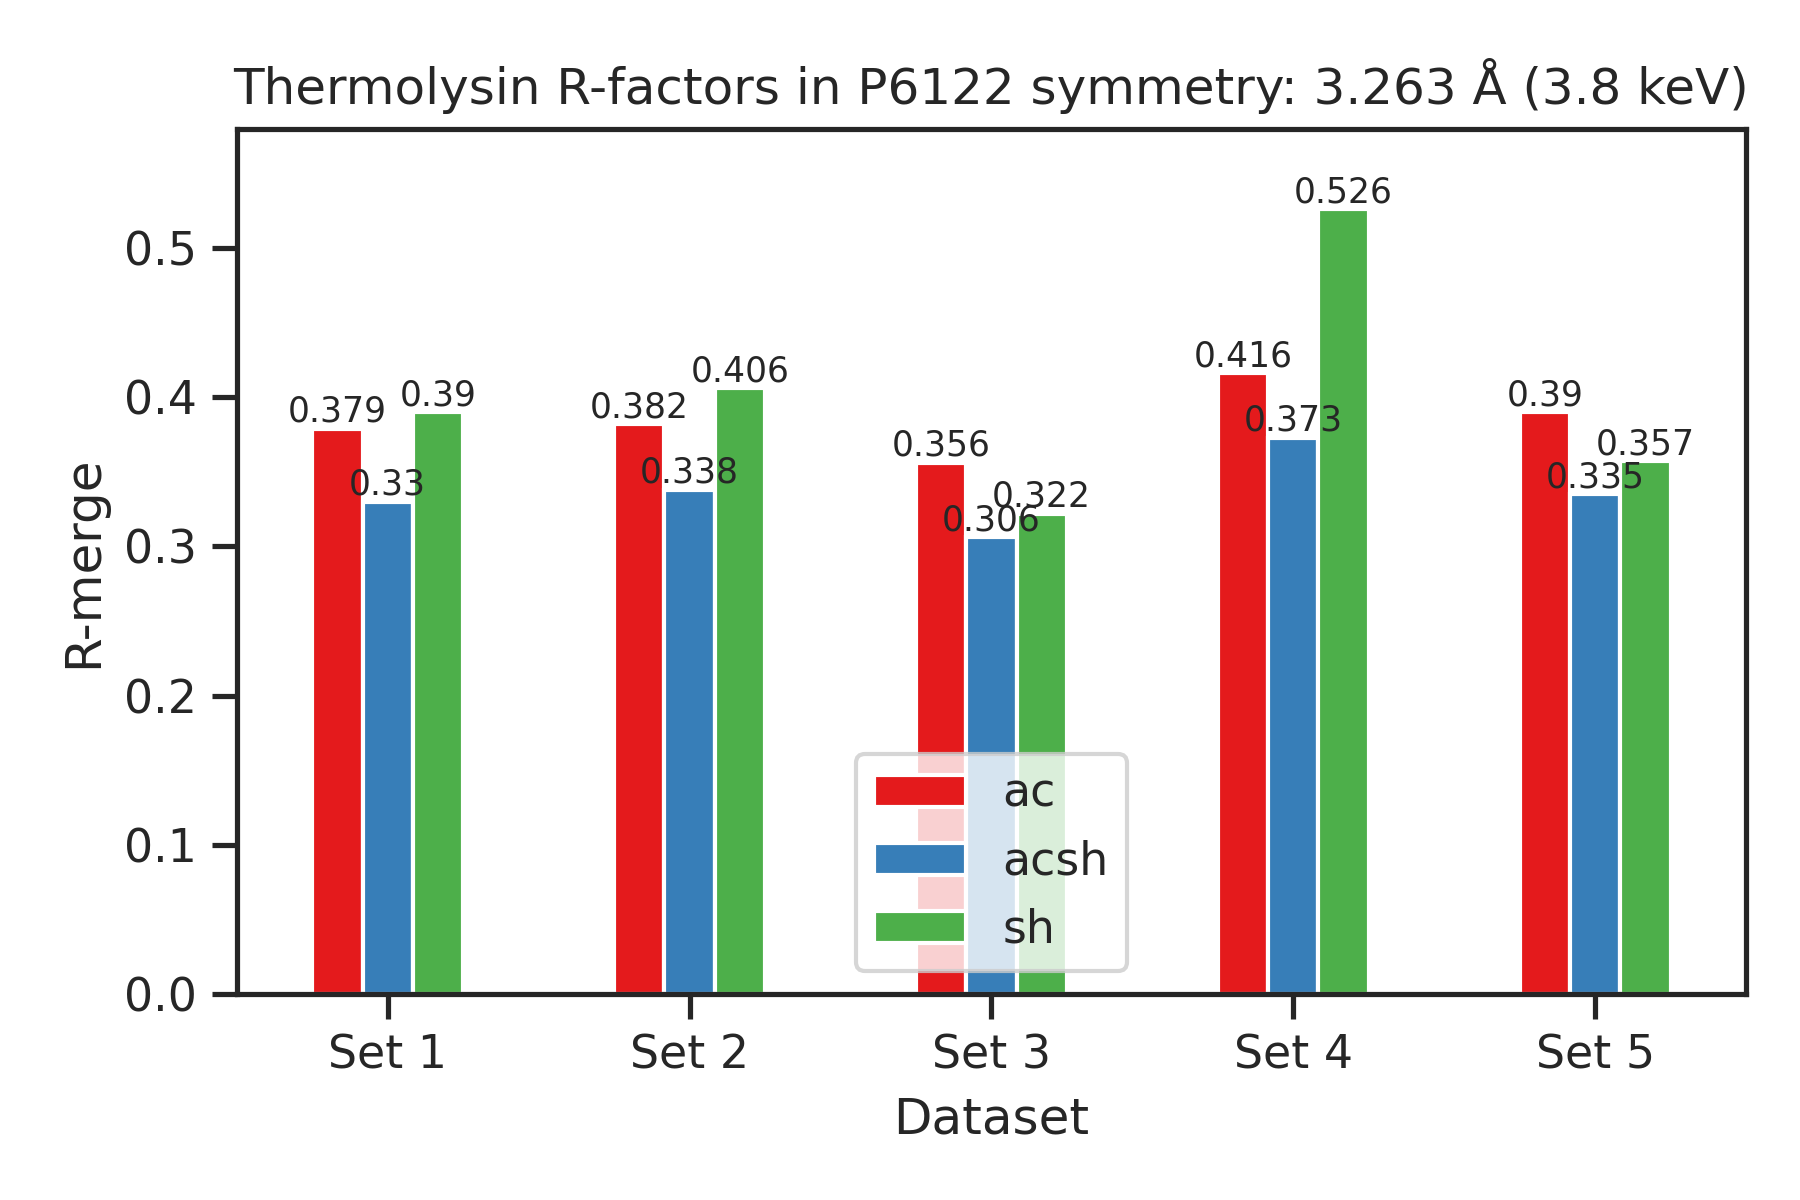
\includegraphics[width = 0.5\textwidth]{plots/exp1/tlys_9_P6122/3p8_rmerges.png}
    \end{tabular}
    \caption{Merging statistics for Thermolysin 1 at 3.8 keV.}
    \label{fig:tlys_9_3p8}
\end{figure}

Taking into account both the increase in $I/\sigma$ and decrease in $R_{merge}$, the merging statistics from Thermolysin 1 showed that \ac{acsh}, which combines tomography with spherical harmonics, was on average the best approach. While this was the case for every dataset of Thermolysin 1, some instances showed only a small improvement compared to \ac{sh}. Likewise, the standalone analytical approach was on average worse than \ac{sh} as well as \ac{acsh}.

Changes in energy are not expected to affect the reflection data in a relevant way; however, energies that were collected subsequently are expected to be more affected by radiation damage from longer exposure to the beam. If segmentation was then performed on a dataset collected early on in the tomography experiment, there can be discrepancies between the analytical model and a more-so radiation-damaged dataset.

%Following collection of reflection data, the AnACor results are used for structure refinement in Dimple, which generates anomalous density peaks for all the detected anomalous atoms and molecules based on the provided model. The results of Thermolysin 1

The merging statistics for Thermolysin 2, seen in \cref{fig:tlys_2_3p0} and \cref{fig:tlys_2_3p5} overwhelmingly show the same trend, with \ac{acsh} being the dominating correction method across all datasets and energies. This was corroborated with the $I/\sigma$ values and the R factors.
%that \ac{acsh} is once again the best correction method
%Results from Thermolysin 2 overwhelmingly show that \ac{acsh} is the dominating correction method, with $I/ \sigma$ highest and the R factors dipping across every dataset.

Thermolysin belongs to the symmetry space group \textit{P}6\textsubscript{1}22. While processing in \textit{P}6\textsubscript{1}22 is therefore needed for obtaining reflection information, high symmetry crystals can still be processed in low symmetry groups, such as \textit{P}\textsubscript{1}, to observe the general merging statistics of the experiment, independent of reflections.

\begin{figure}[h]
    \centering
    \begin{tabular}{cc}
    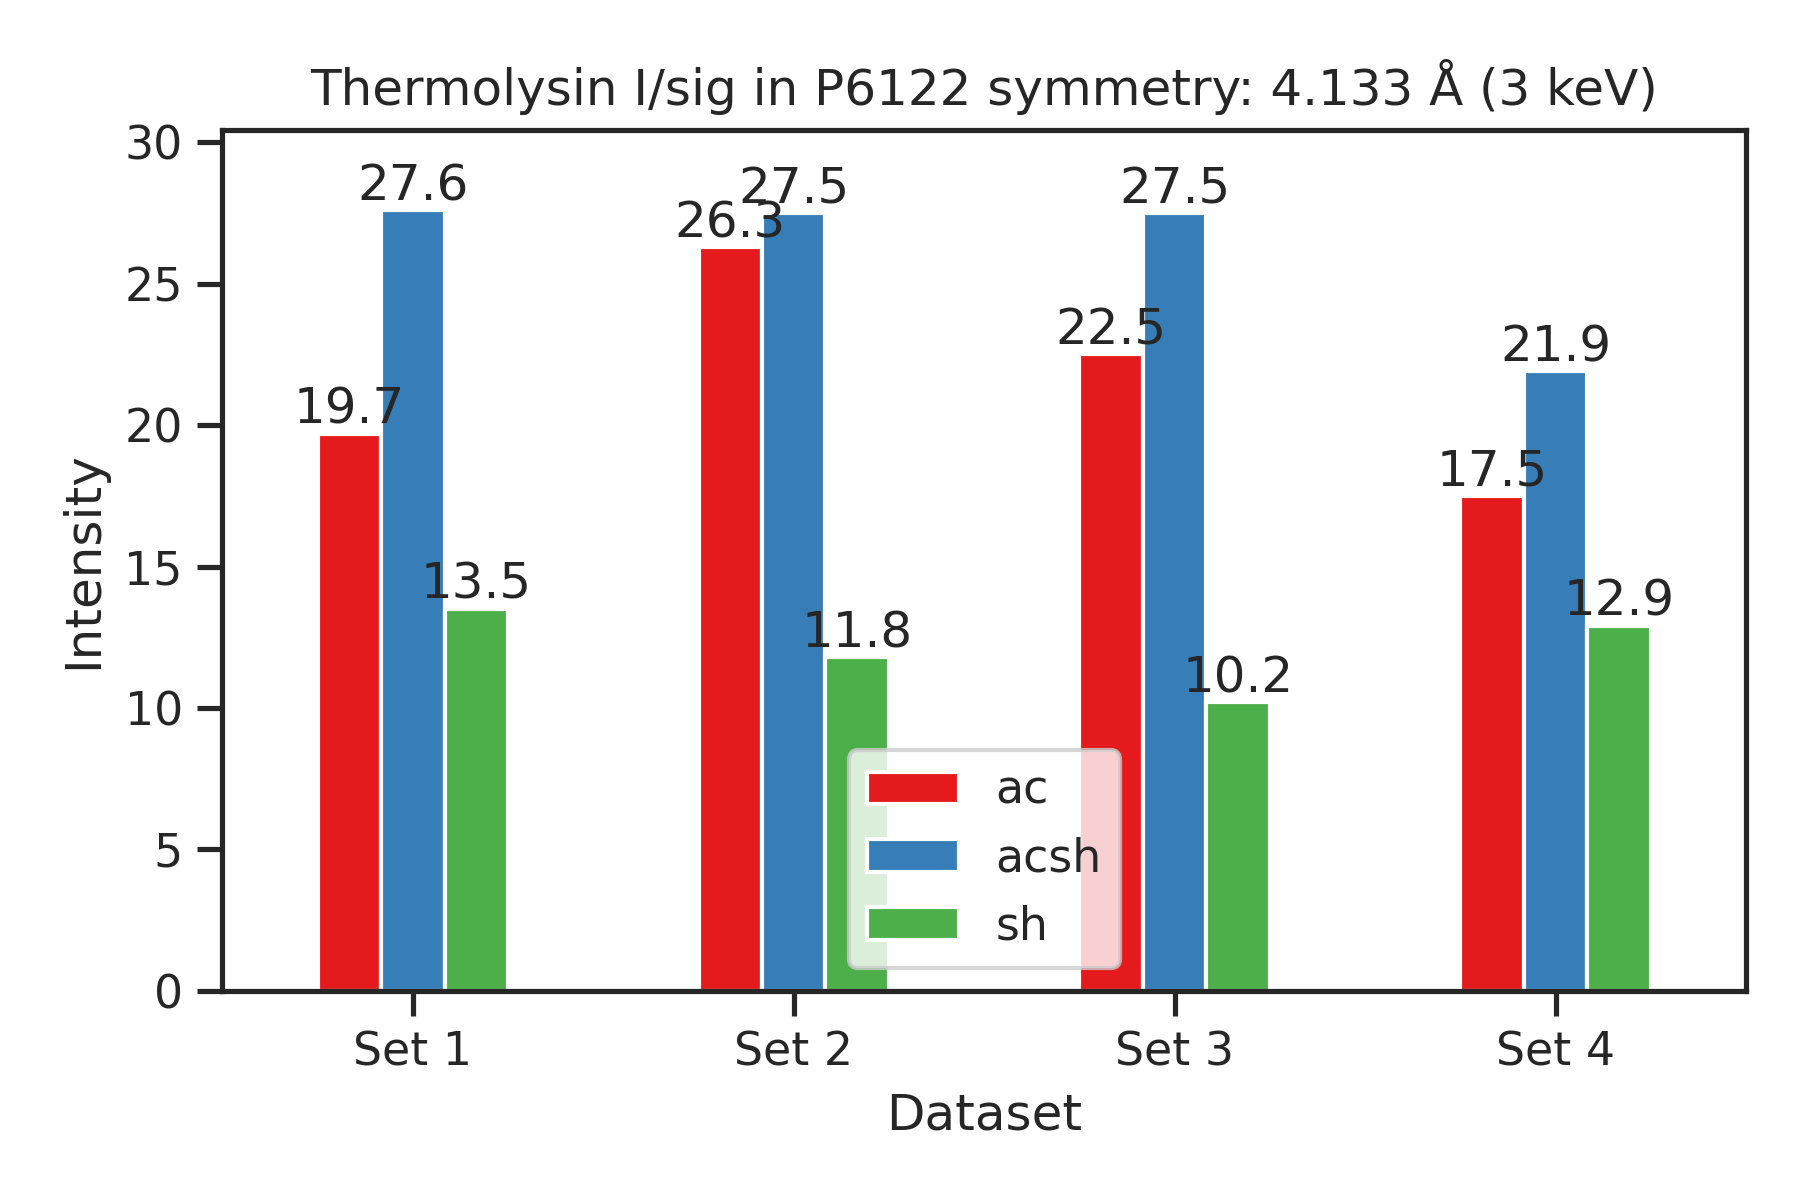
\includegraphics[width = 0.5\textwidth]{plots/exp1/tlys_2_P6122/3p0_I_over_sigma.png} & 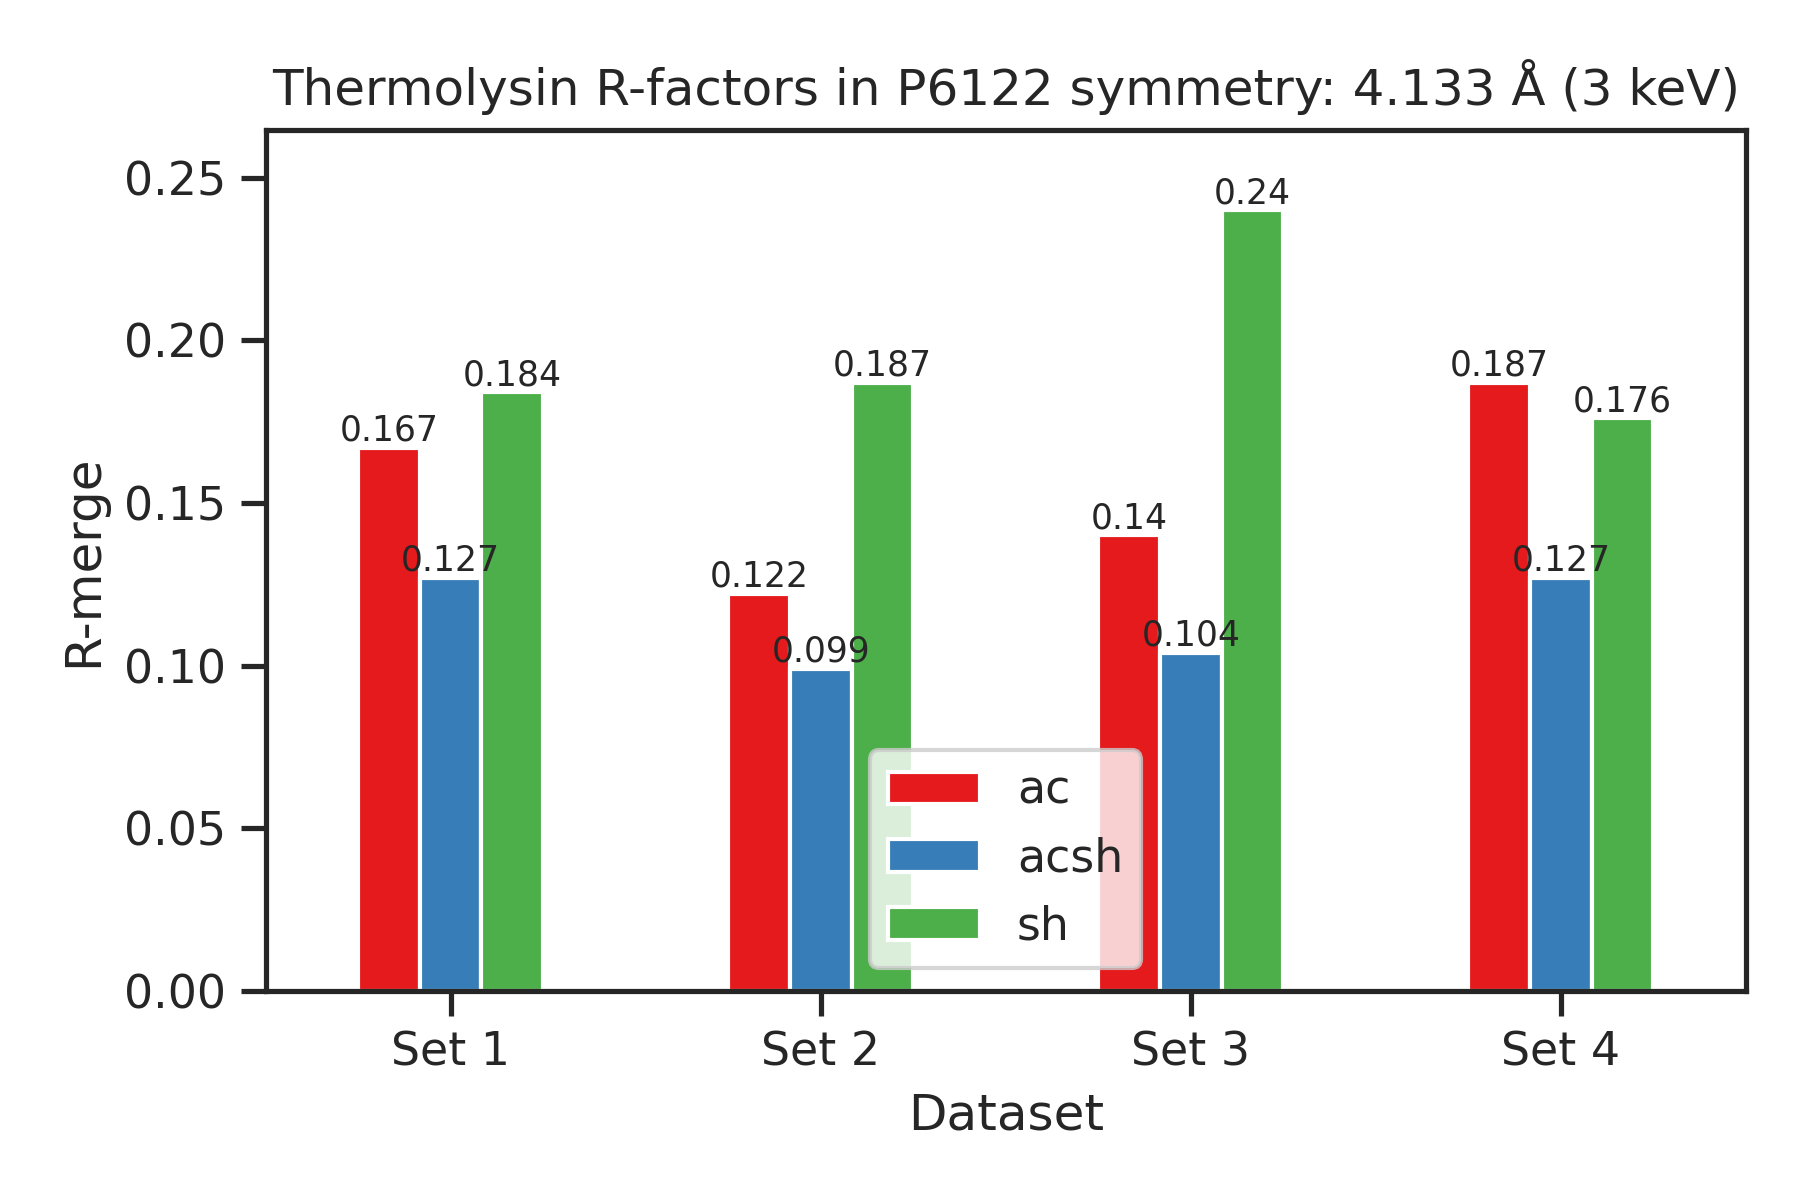
\includegraphics[width = 0.5\textwidth]{plots/exp1/tlys_2_P6122/3p0_rmerges.png}
    \end{tabular}
    \caption{Merging statistics for Thermolysin 2 at 3.0 keV.}
    \label{fig:tlys_2_3p0}
\end{figure}

\begin{figure}[h]
    \centering
    \begin{tabular}{cc}
    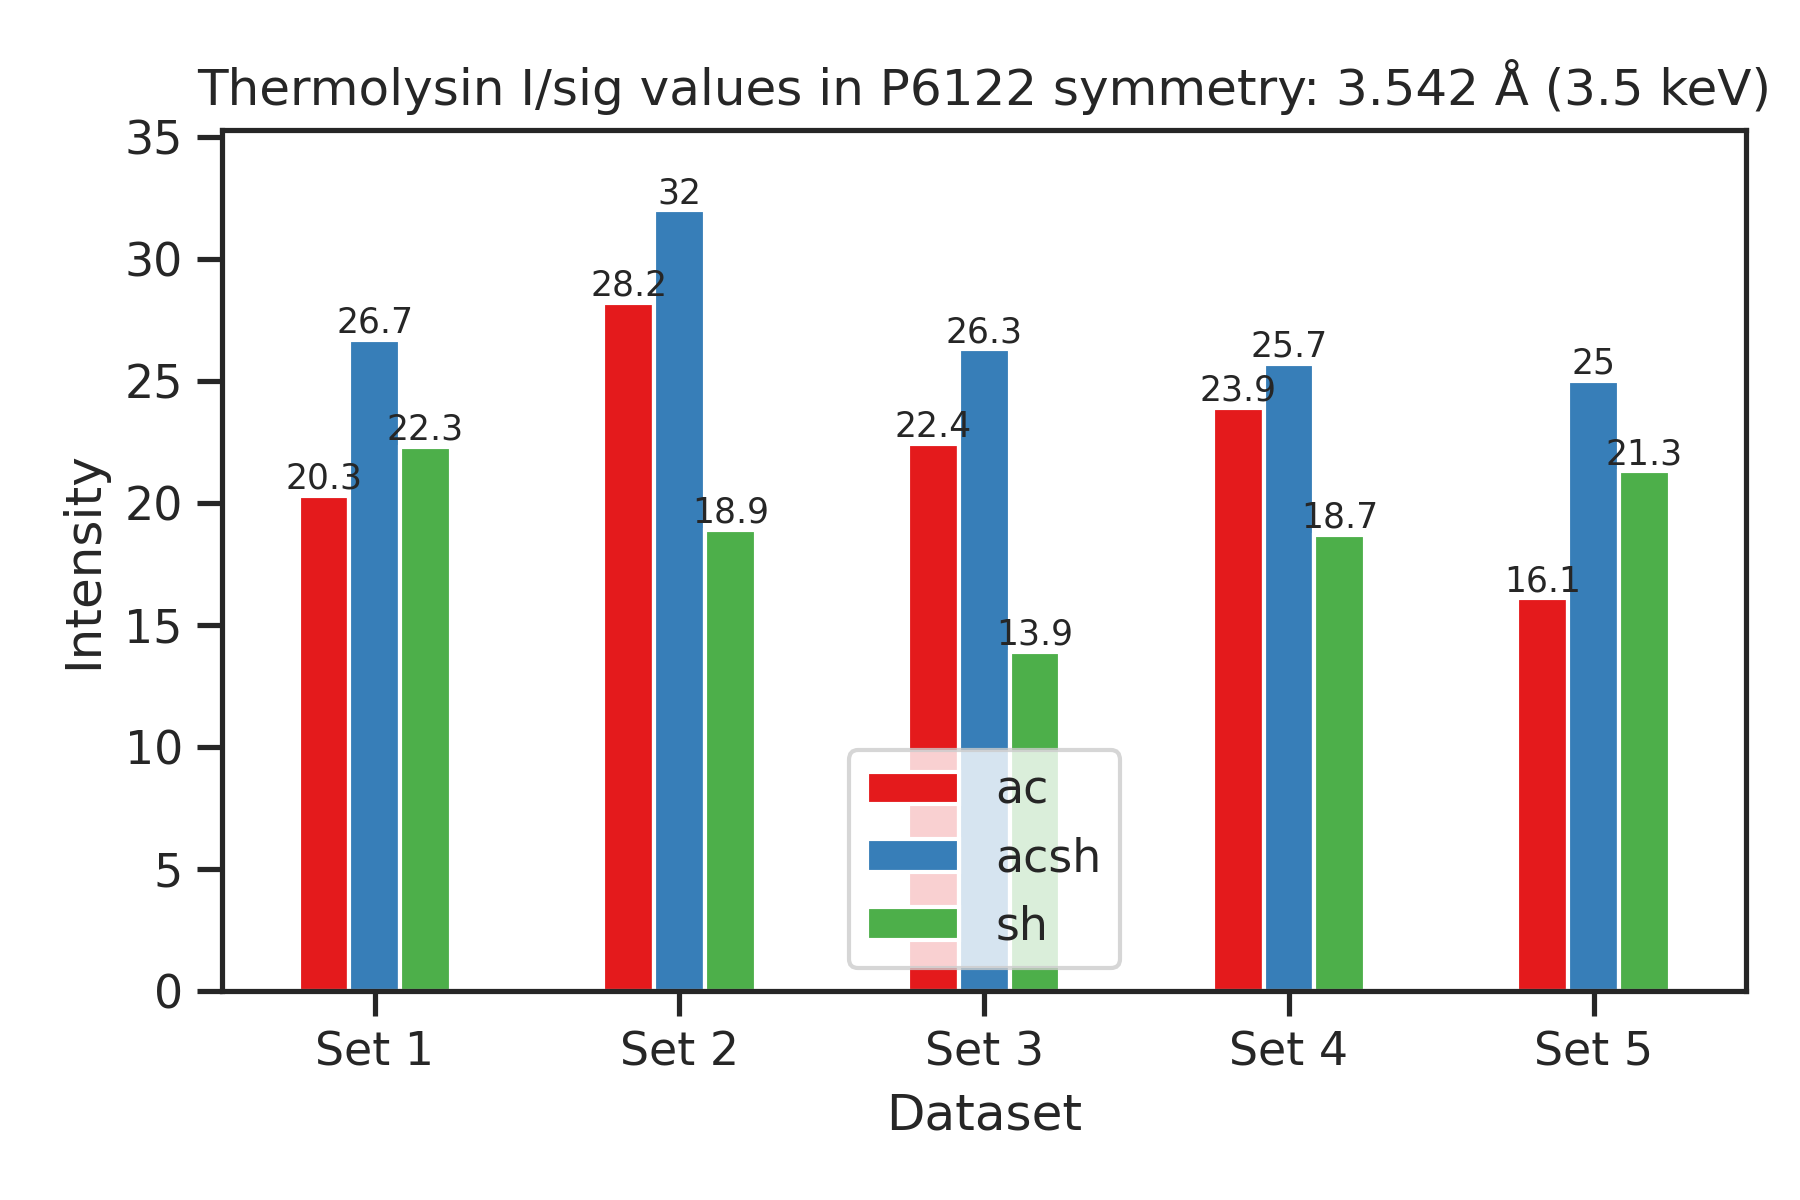
\includegraphics[width = 0.5\textwidth]{plots/exp1/tlys_2_P6122/3p5_I_over_sigma.png} & 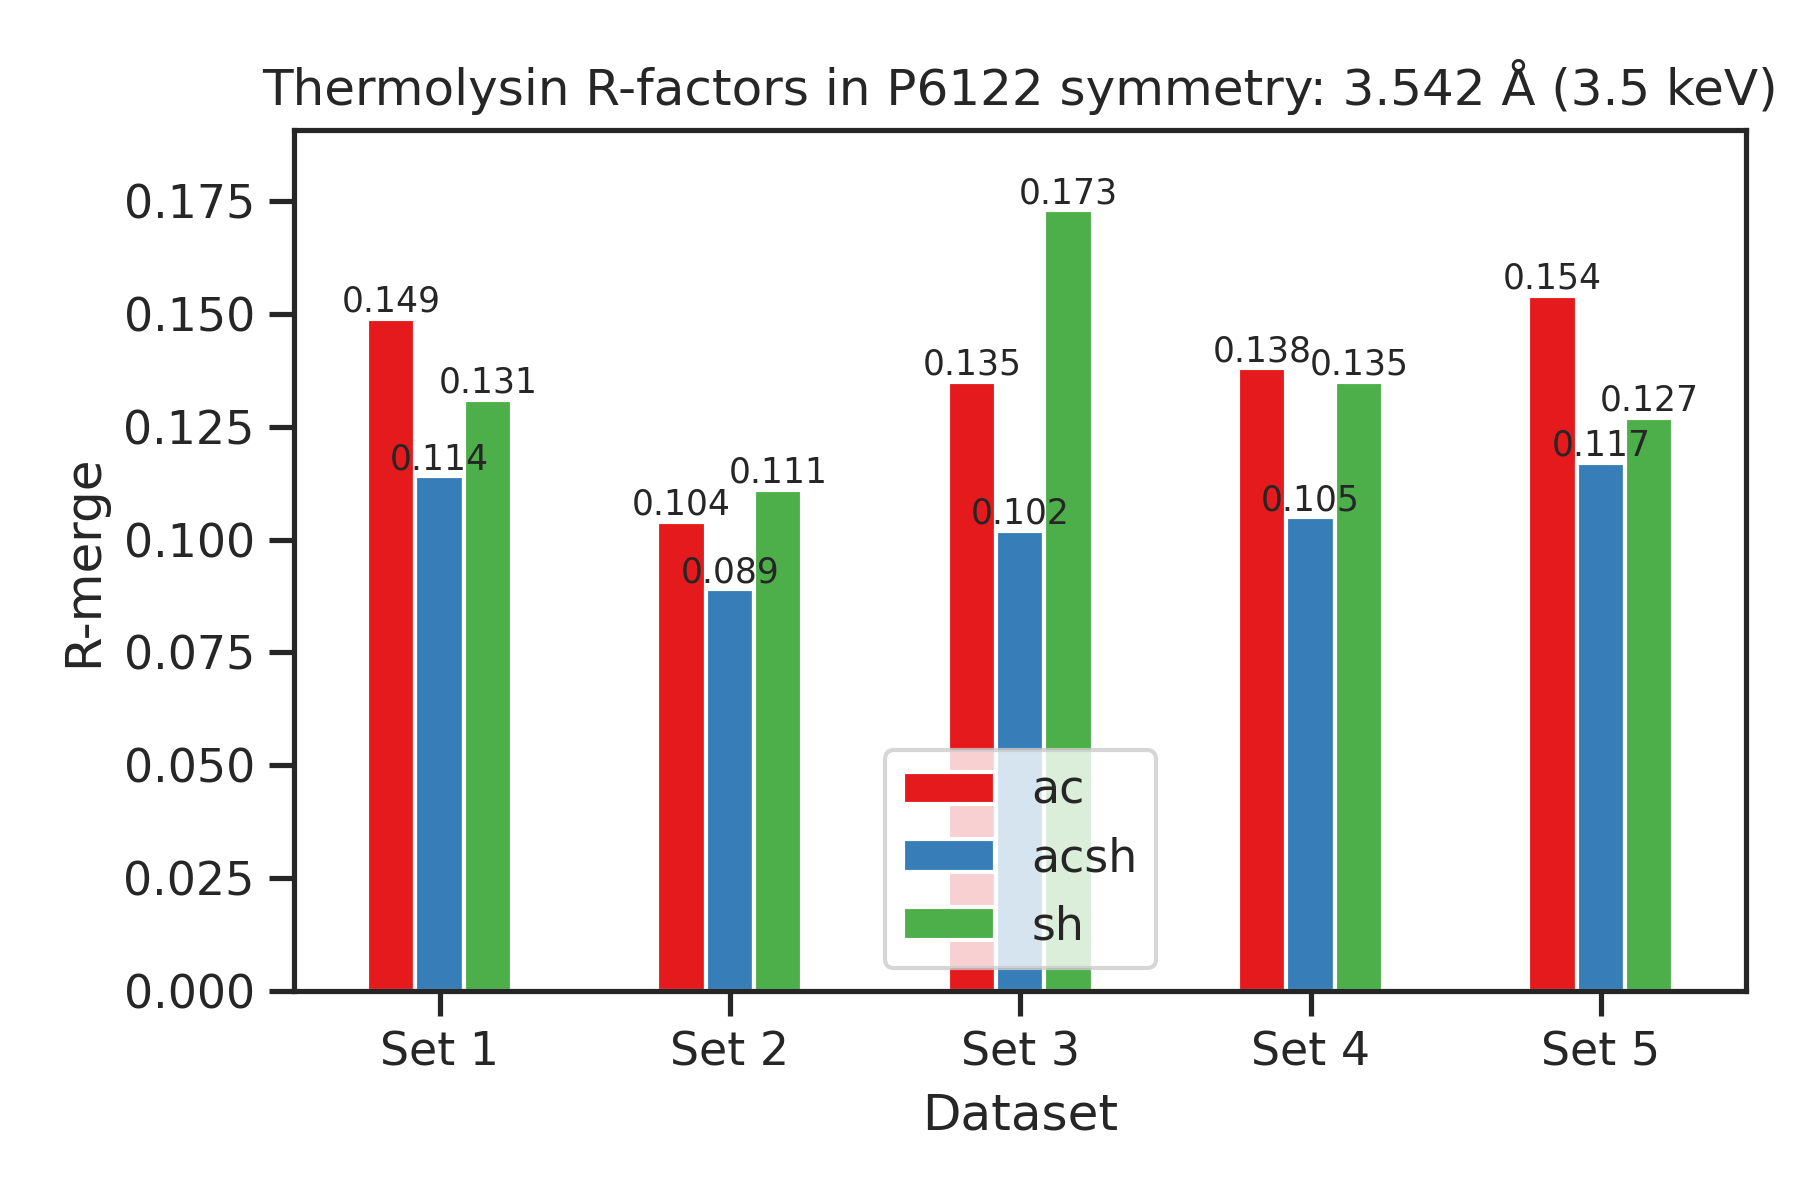
\includegraphics[width = 0.5\textwidth]{plots/exp1/tlys_2_P6122/3p5_rmerges.png}
    \end{tabular}
    \caption{Merging statistics for Thermolysin 2 at 3.5 keV.}
    \label{fig:tlys_2_3p5}
\end{figure}

Following collection of reflection data, the AnACor results are used for structure refinement in Dimple to generate anomalous density peaks for all the detected anomalous atoms and molecules, based on the provided model. In thermolysin, the relevant anomalous groups are two conformations of methionine (205 and 120), and a zinc atom. The results of Thermolysin 2 are shown in \cref{fig:tlys2_met_peaks_3p0, fig:tlys2_met_peaks_3p5, fig:tlys2_zn_peaks}.% and \cref{fig:tlys2_met_peaks_3p5}.

Datasets across the same energy processed in P\textsubscript{1} were additionally merged to increase the multiplicity of the low symmetry space group, and the results of processing Thermolysin 1 and Thermolysin 2 in P\textsubscript{1} repeat the same trend seen for \textit{P}6\textsubscript{1}22.

\begin{figure}[h]
    \centering
    \begin{tabular}{cc}
    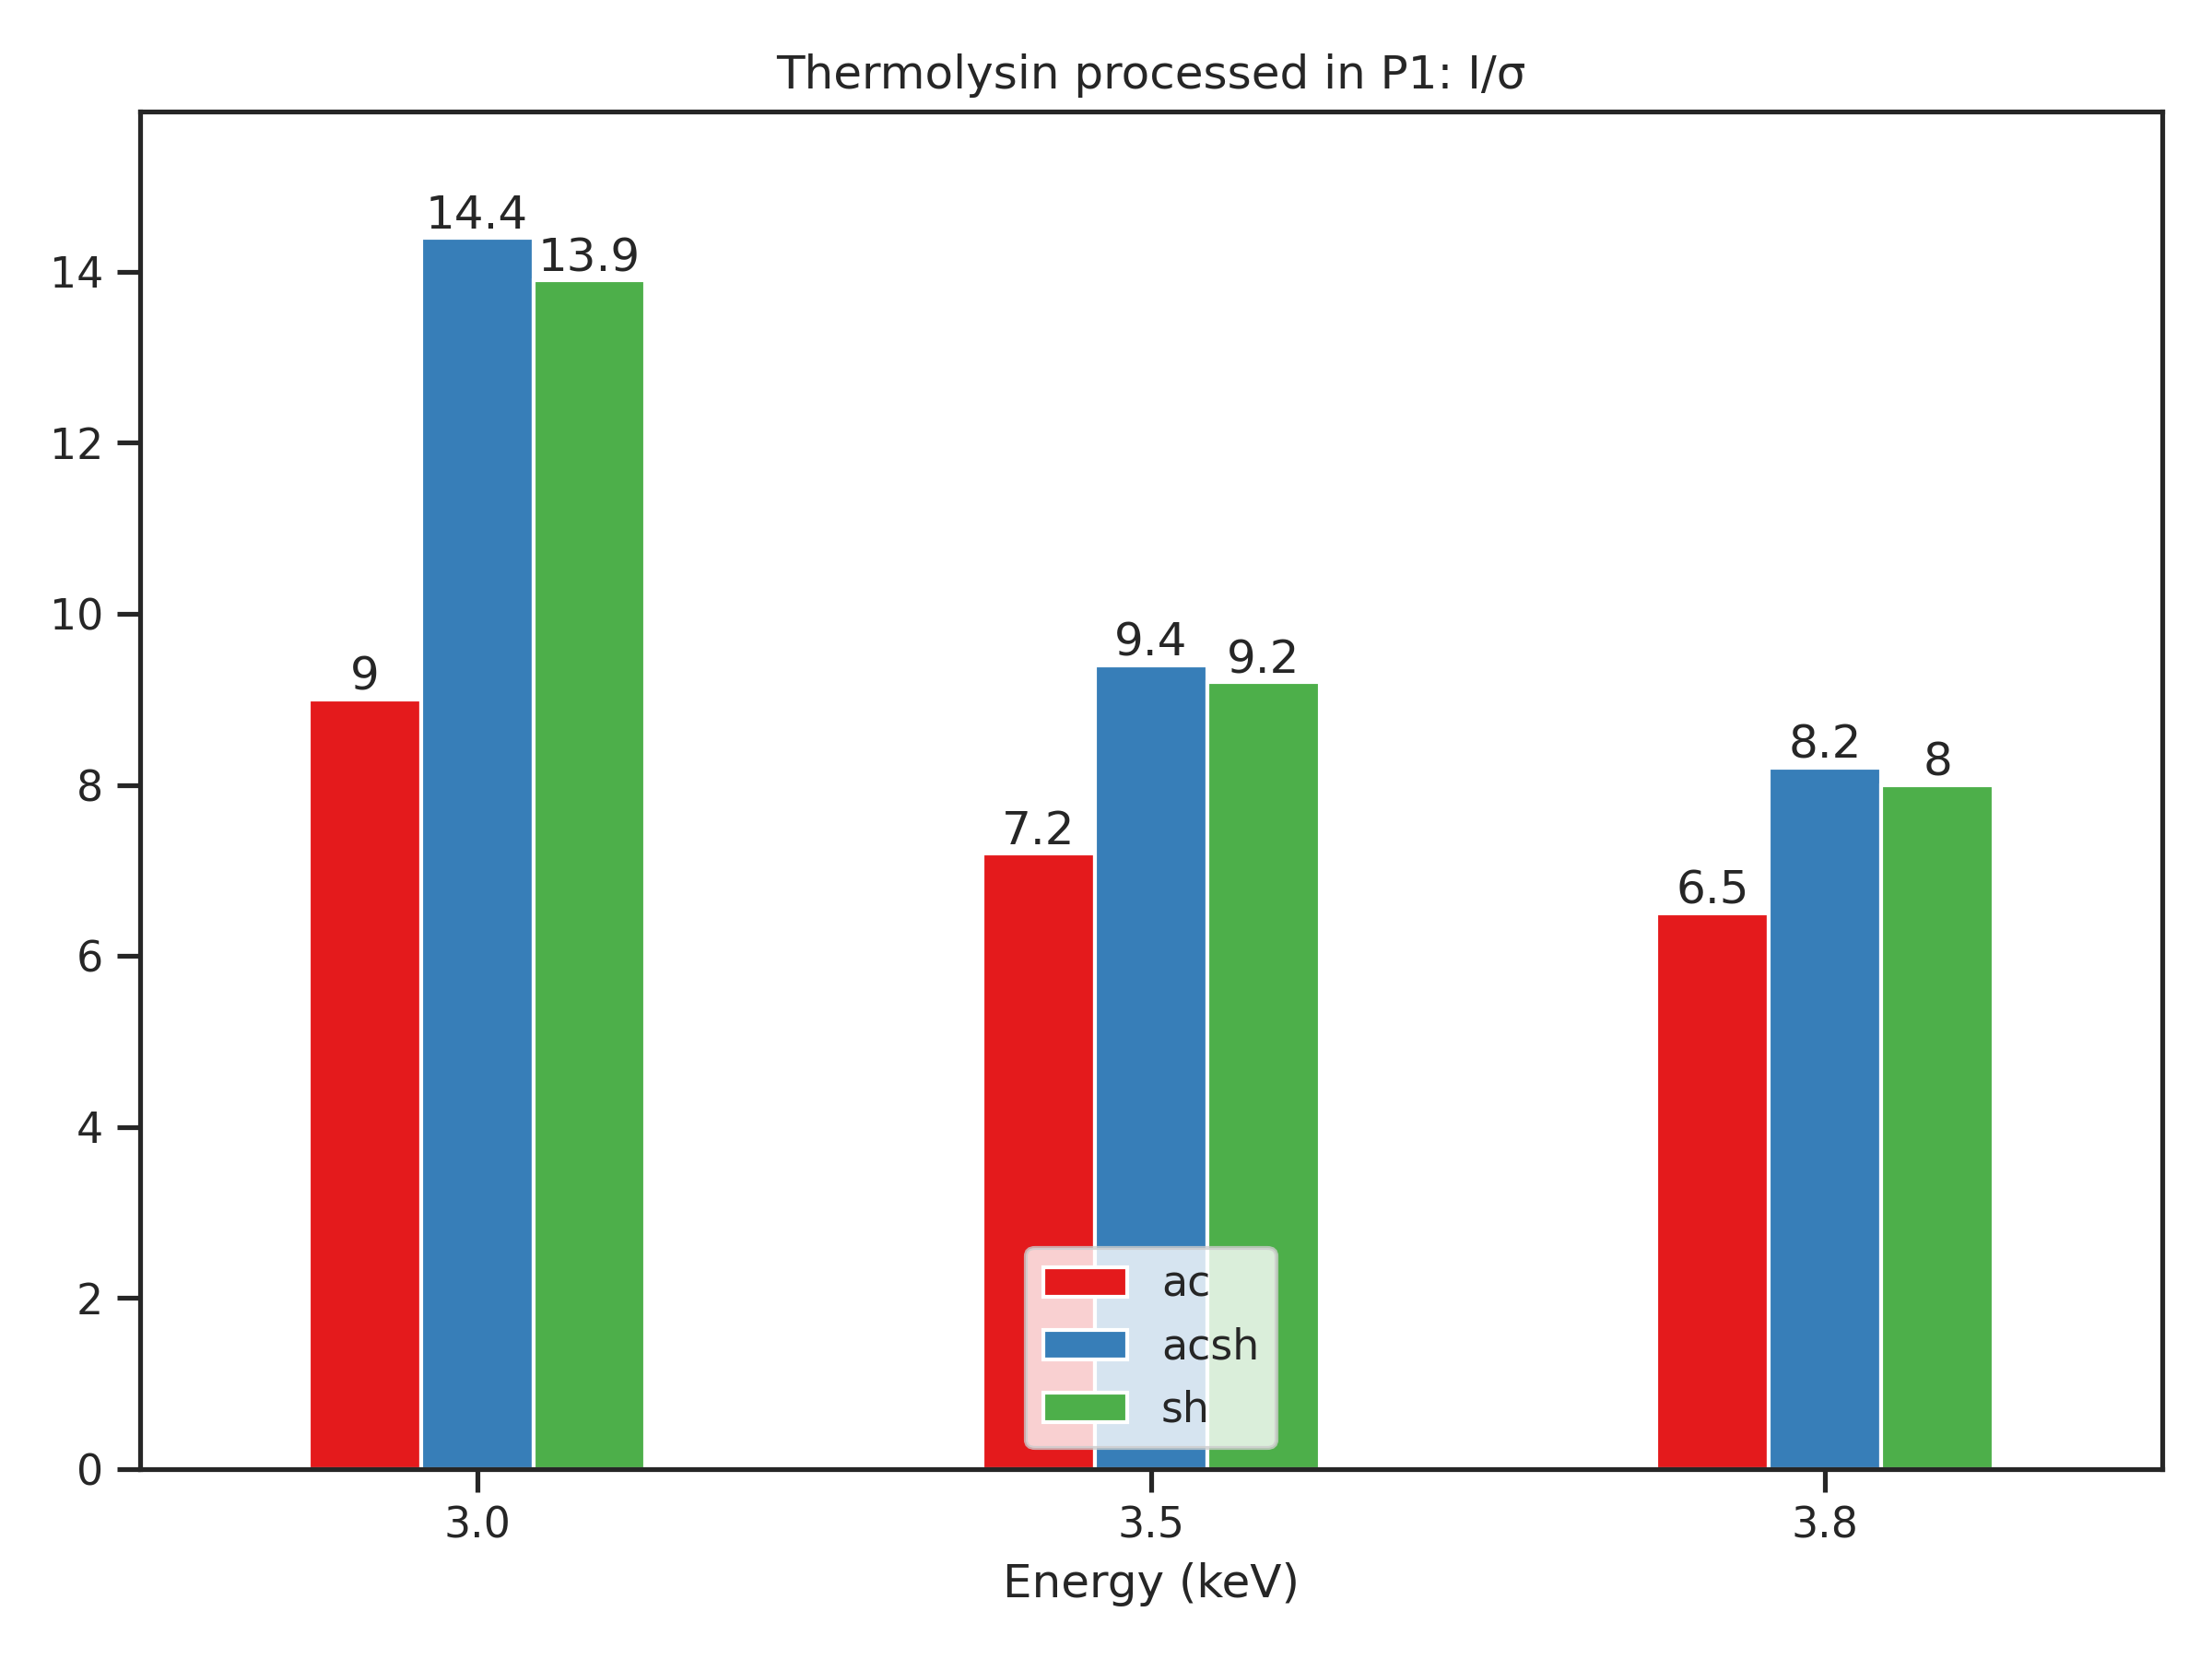
\includegraphics[width = 0.5\textwidth]{plots/exp1/tlys_9_P1/I_over_sigma.png} & 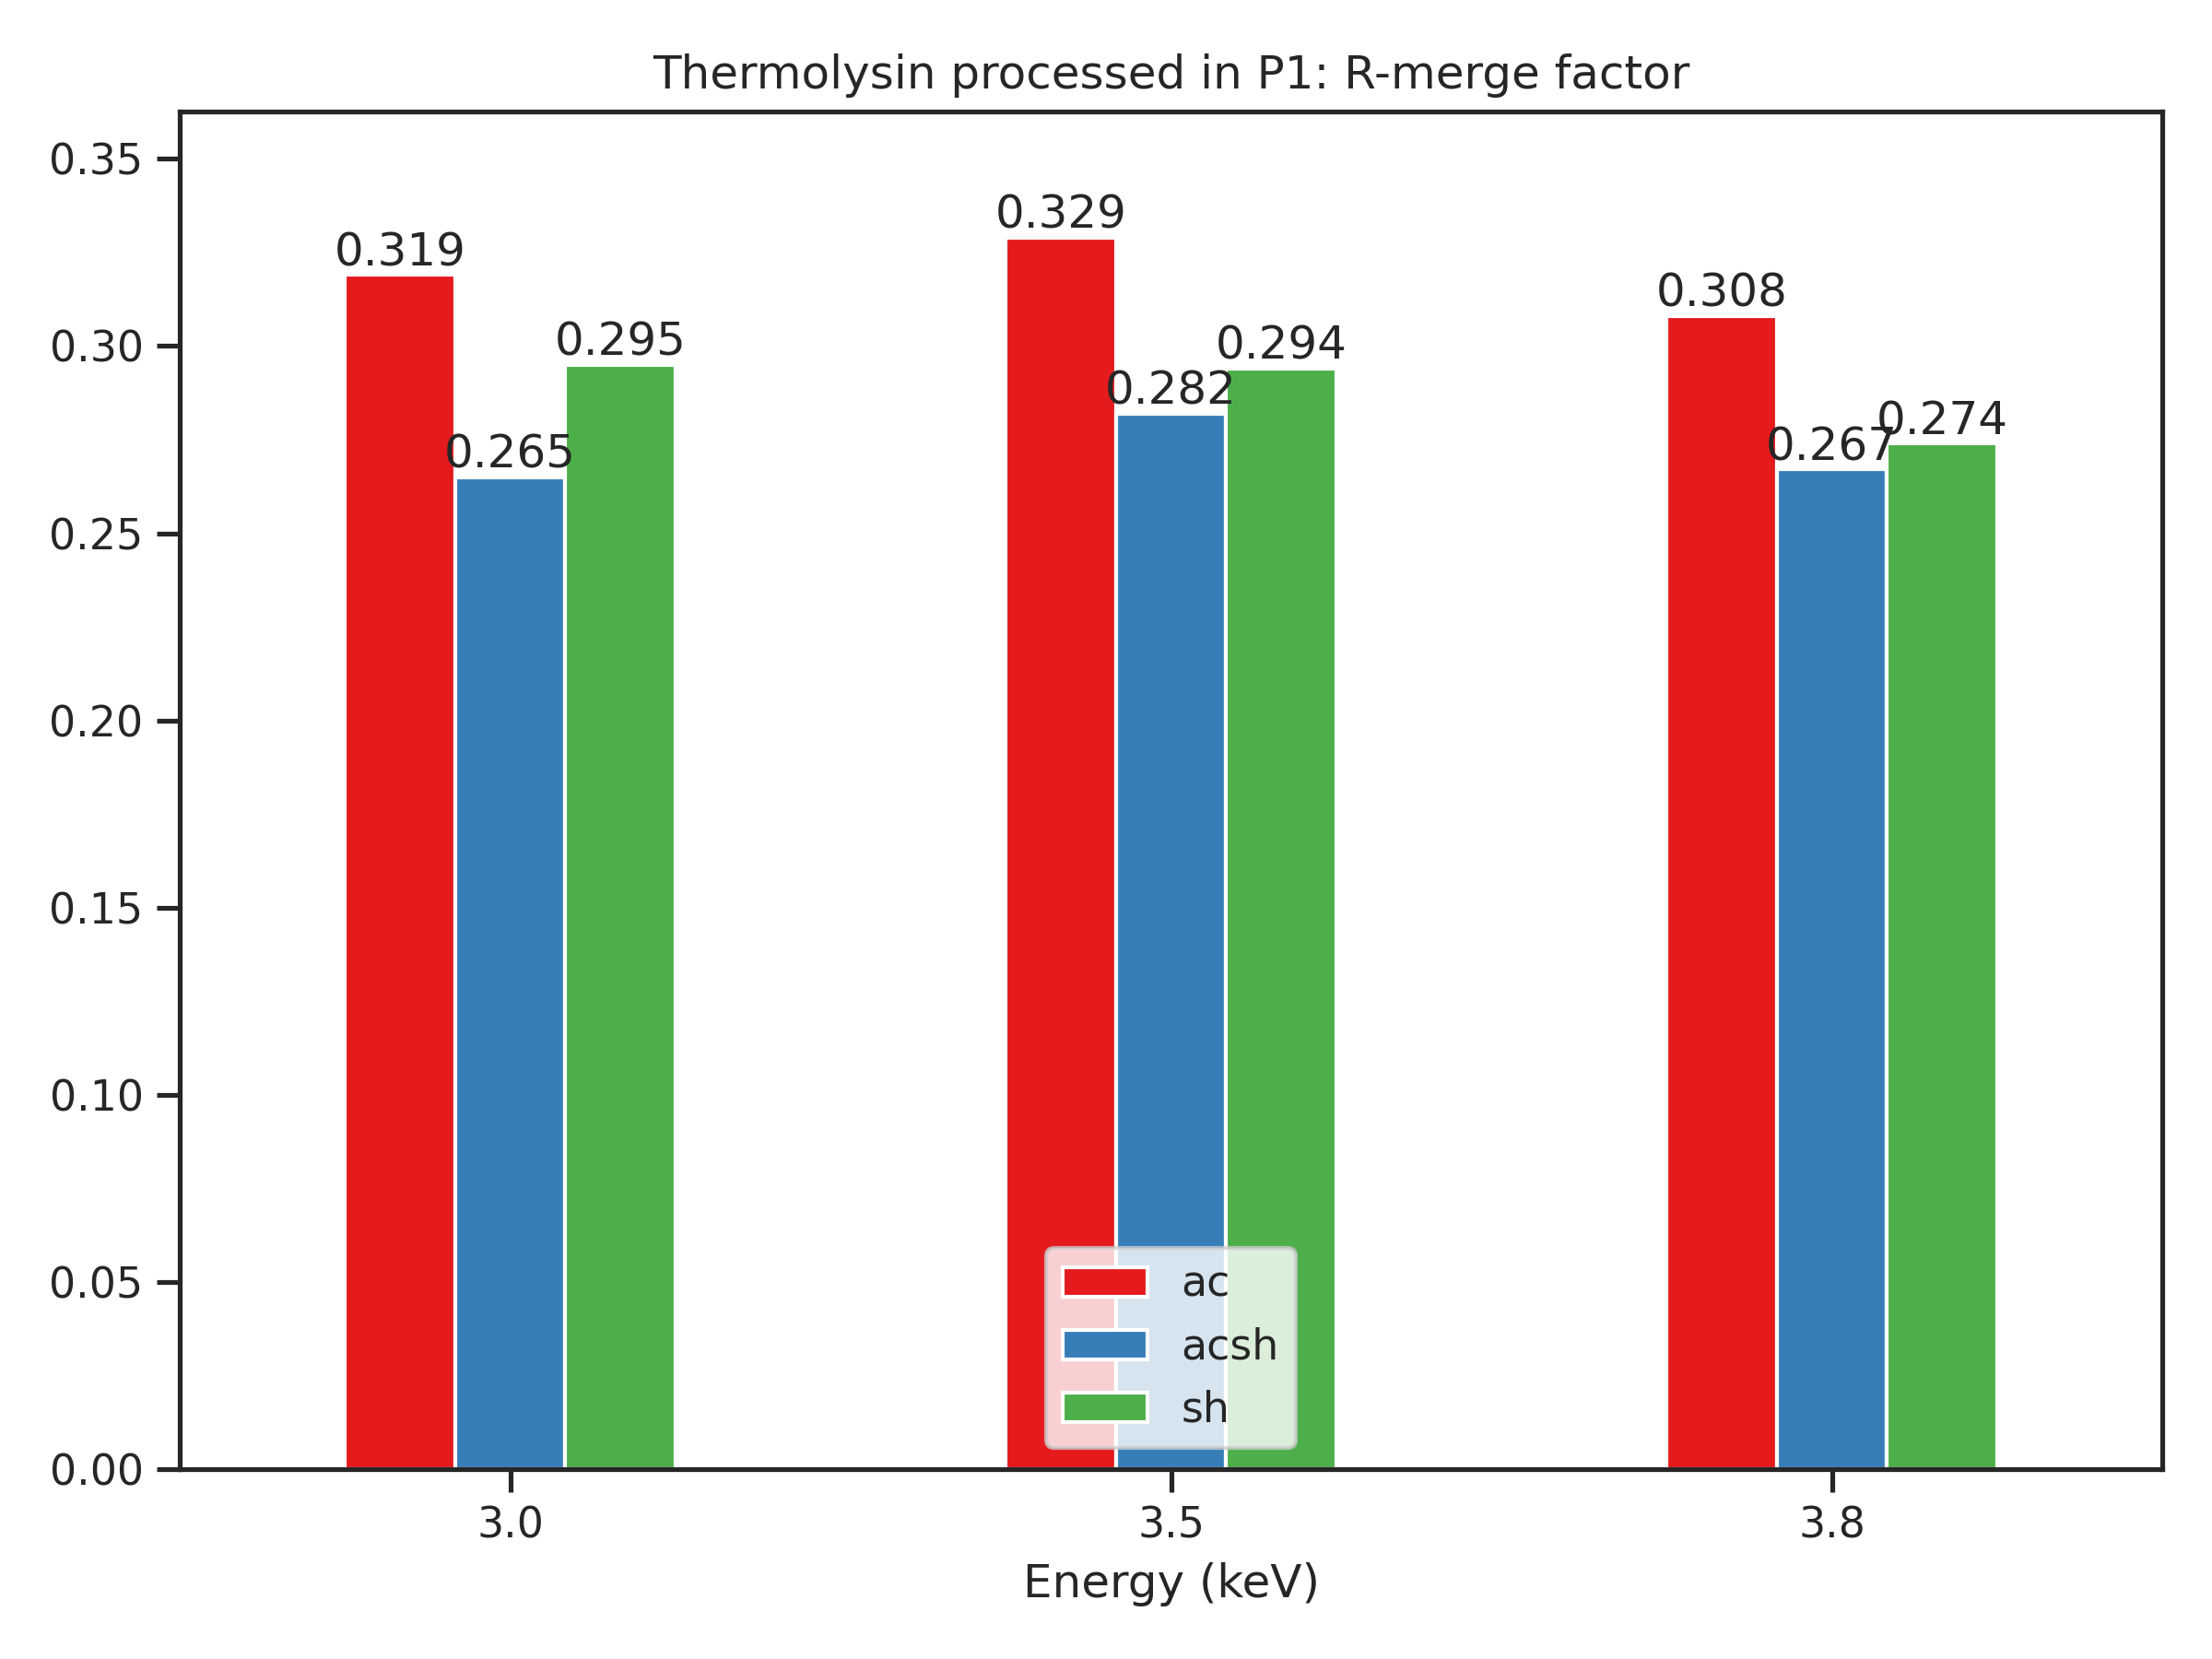
\includegraphics[width = 0.5\textwidth]{plots/exp1/tlys_9_P1/rmerges.png}
    \end{tabular}
    \caption{Caption}
    \label{fig:tlys_2_p6}
\end{figure}

\begin{figure}[h]
    \centering
    \begin{tabular}{cc}
    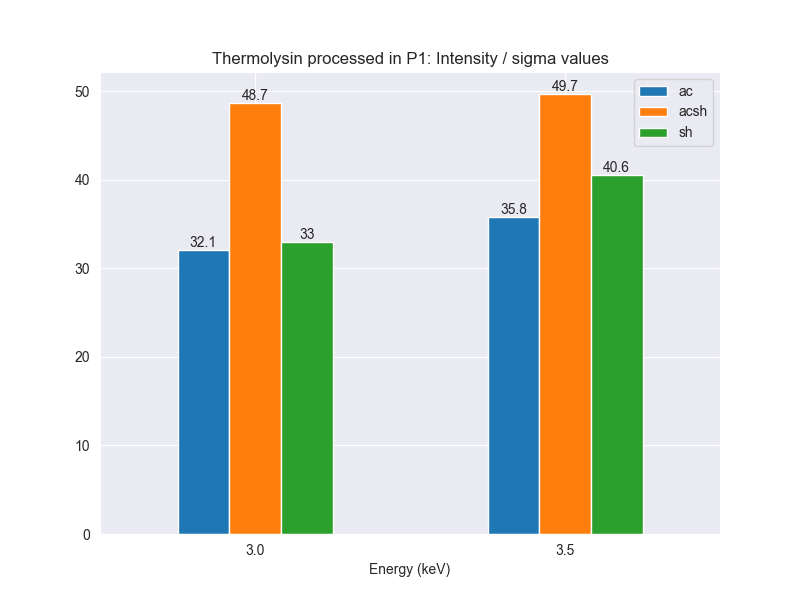
\includegraphics[width = 0.5\textwidth]{plots/exp1/tlys_2_P1/I_over_sigma.png} & 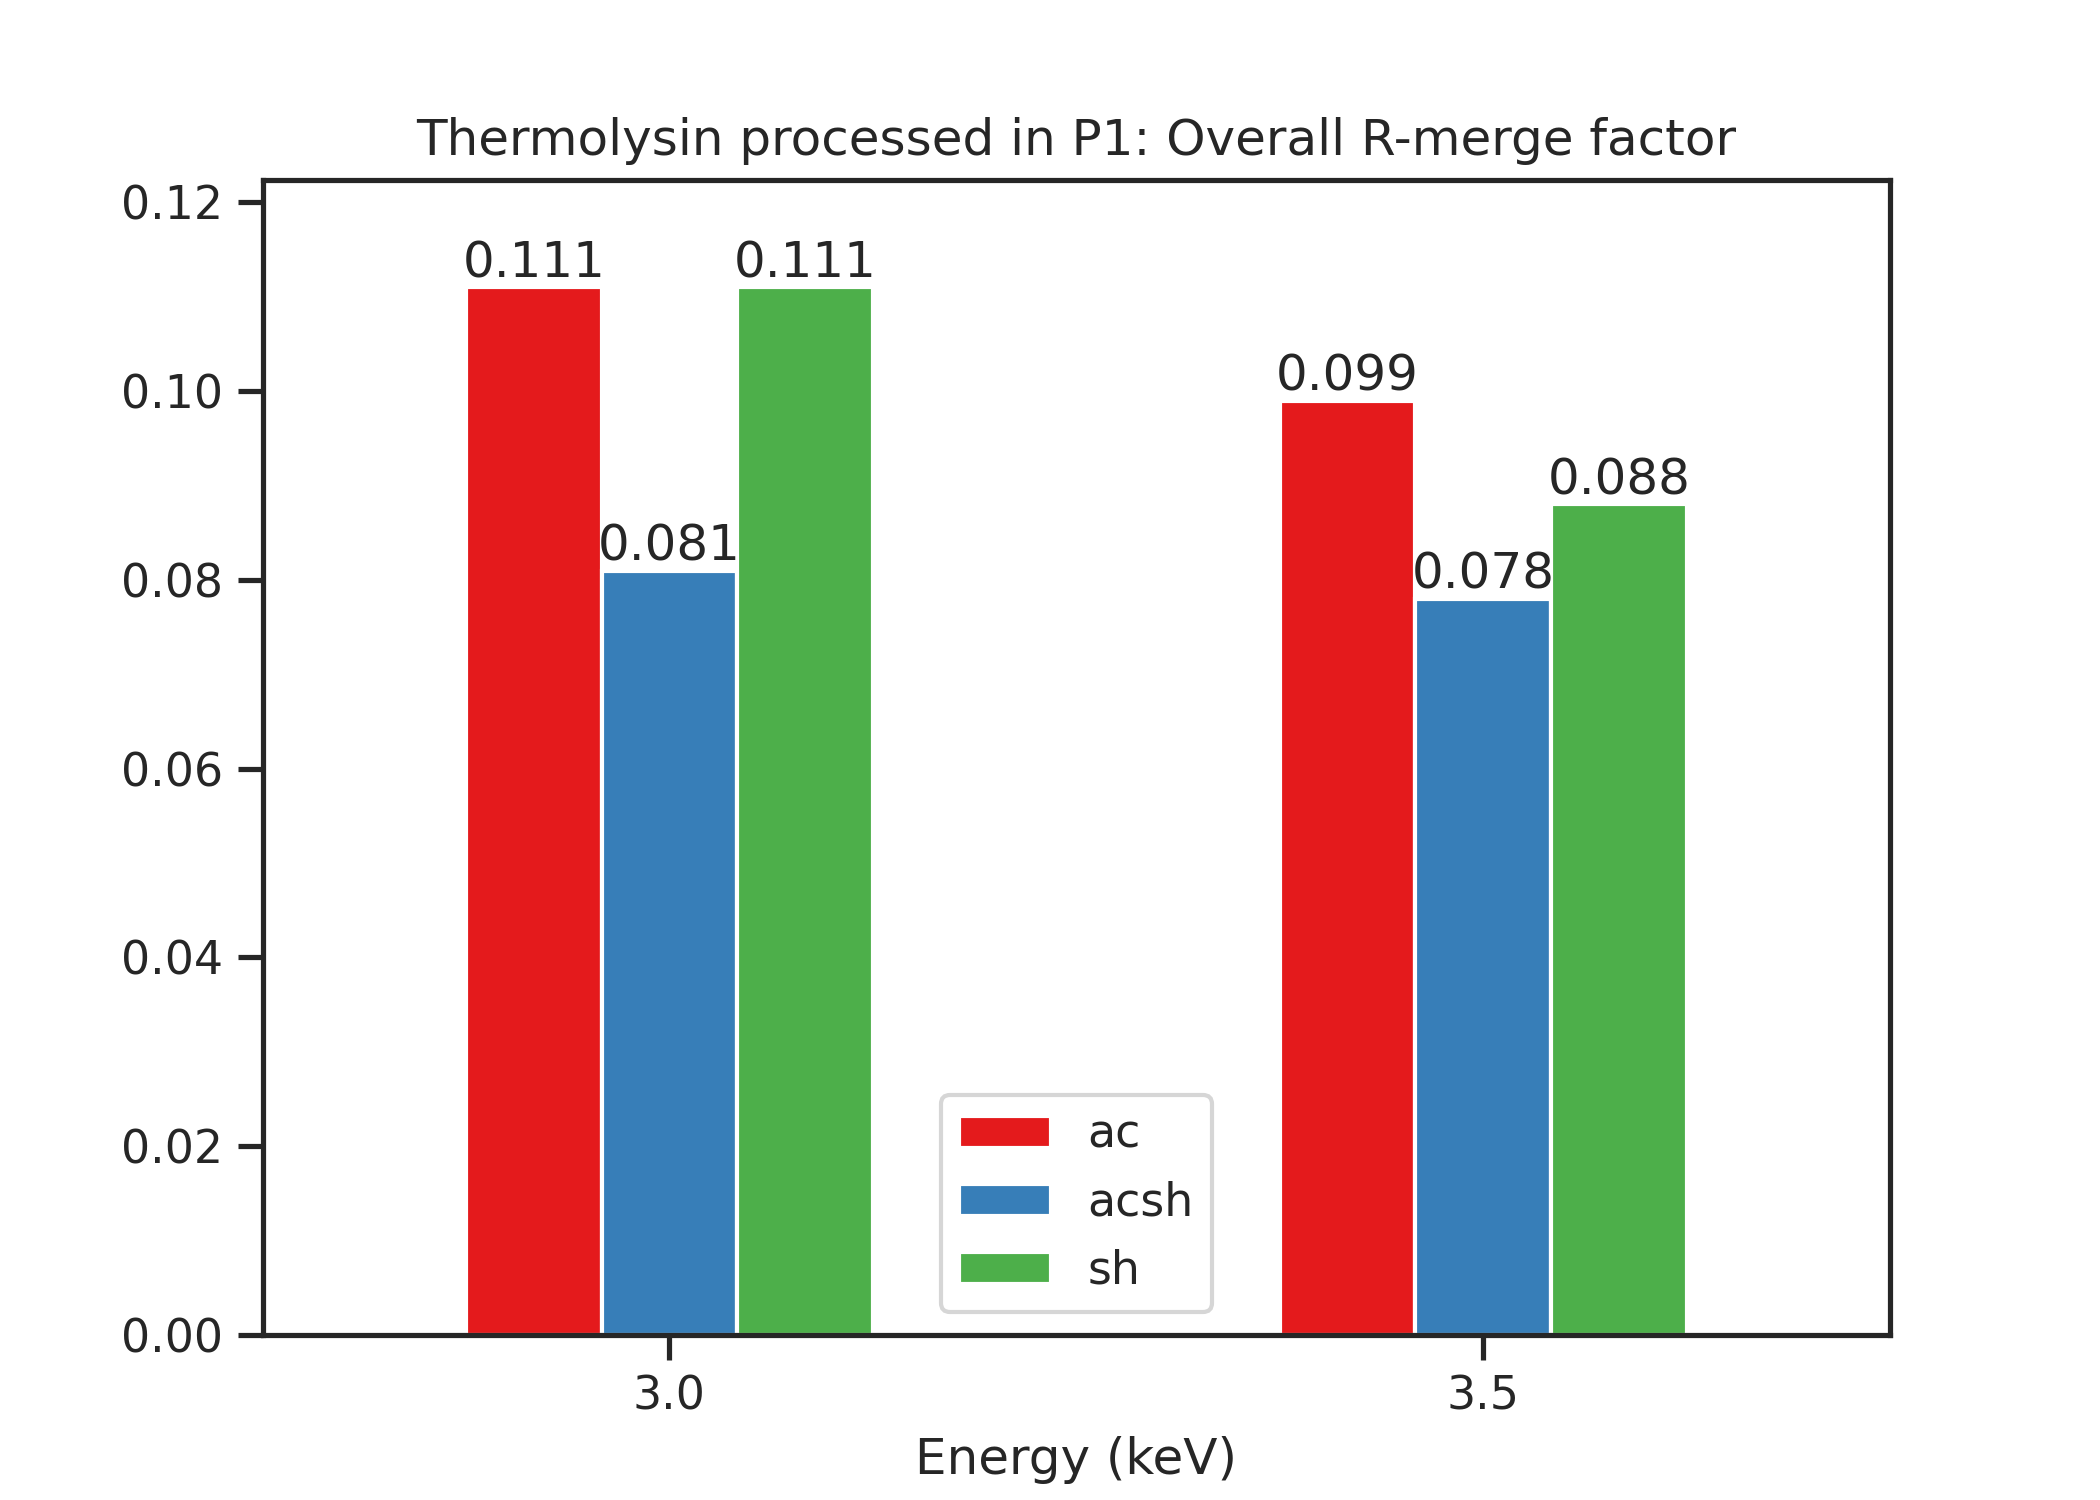
\includegraphics[width = 0.5\textwidth]{plots/exp1/tlys_2_P1/rmerges.png}
    \end{tabular}
    \caption{Caption}
    \label{fig:tlys_2_p6}
\end{figure}

\subsection{Analytically-corrected Tomography data in $f"$-refinement for ion identification}

%As of this year, I23 has established a new method of ion identification using anomalous scattering known as f" refinement. This protocol uses a programme known as Phenix which has a feature for estimating the f' and f" values of a given element based on the (mtz and pdb) of the collected crystal data. The f"-refinement is becoming a routinely-used feature of ion identification due to the long wavelength capabilities of the beamline. 

The reflection data from Thermolysin 2 that was produced across all three correction methods in the prior experiment were then used in the Phenix in the platform known as \textit{phenix.refine}. This platform allows for the refinement of absorption parameters $f'$ and $f"$ based on the reflection data and \textit{pdb} structure provided. As described in the methodology, the first stage of \textit{phenix.refine} uses the reflection data provided to produce a modified version of the molecular structure in \textit{pdb} format. This updated molecular structure is then used in the second stage with the same reflection data to estimate the theoretical $f'$ and $f"$ values of specified atoms that are believed to be in the structure. In the case of this experiment, $f'$ was fixed to its theoretical value for a given atom and energy, allowing for an experimental $f"$ to be refined. This value is then corroborated with the theoretical value to determine whether the atom type can be correctly identified.% test the ability of identifying atoms of sulphur and zinc in the crystal by determining their $f"$ peak.


\begin{figure}[h]
    \centering
    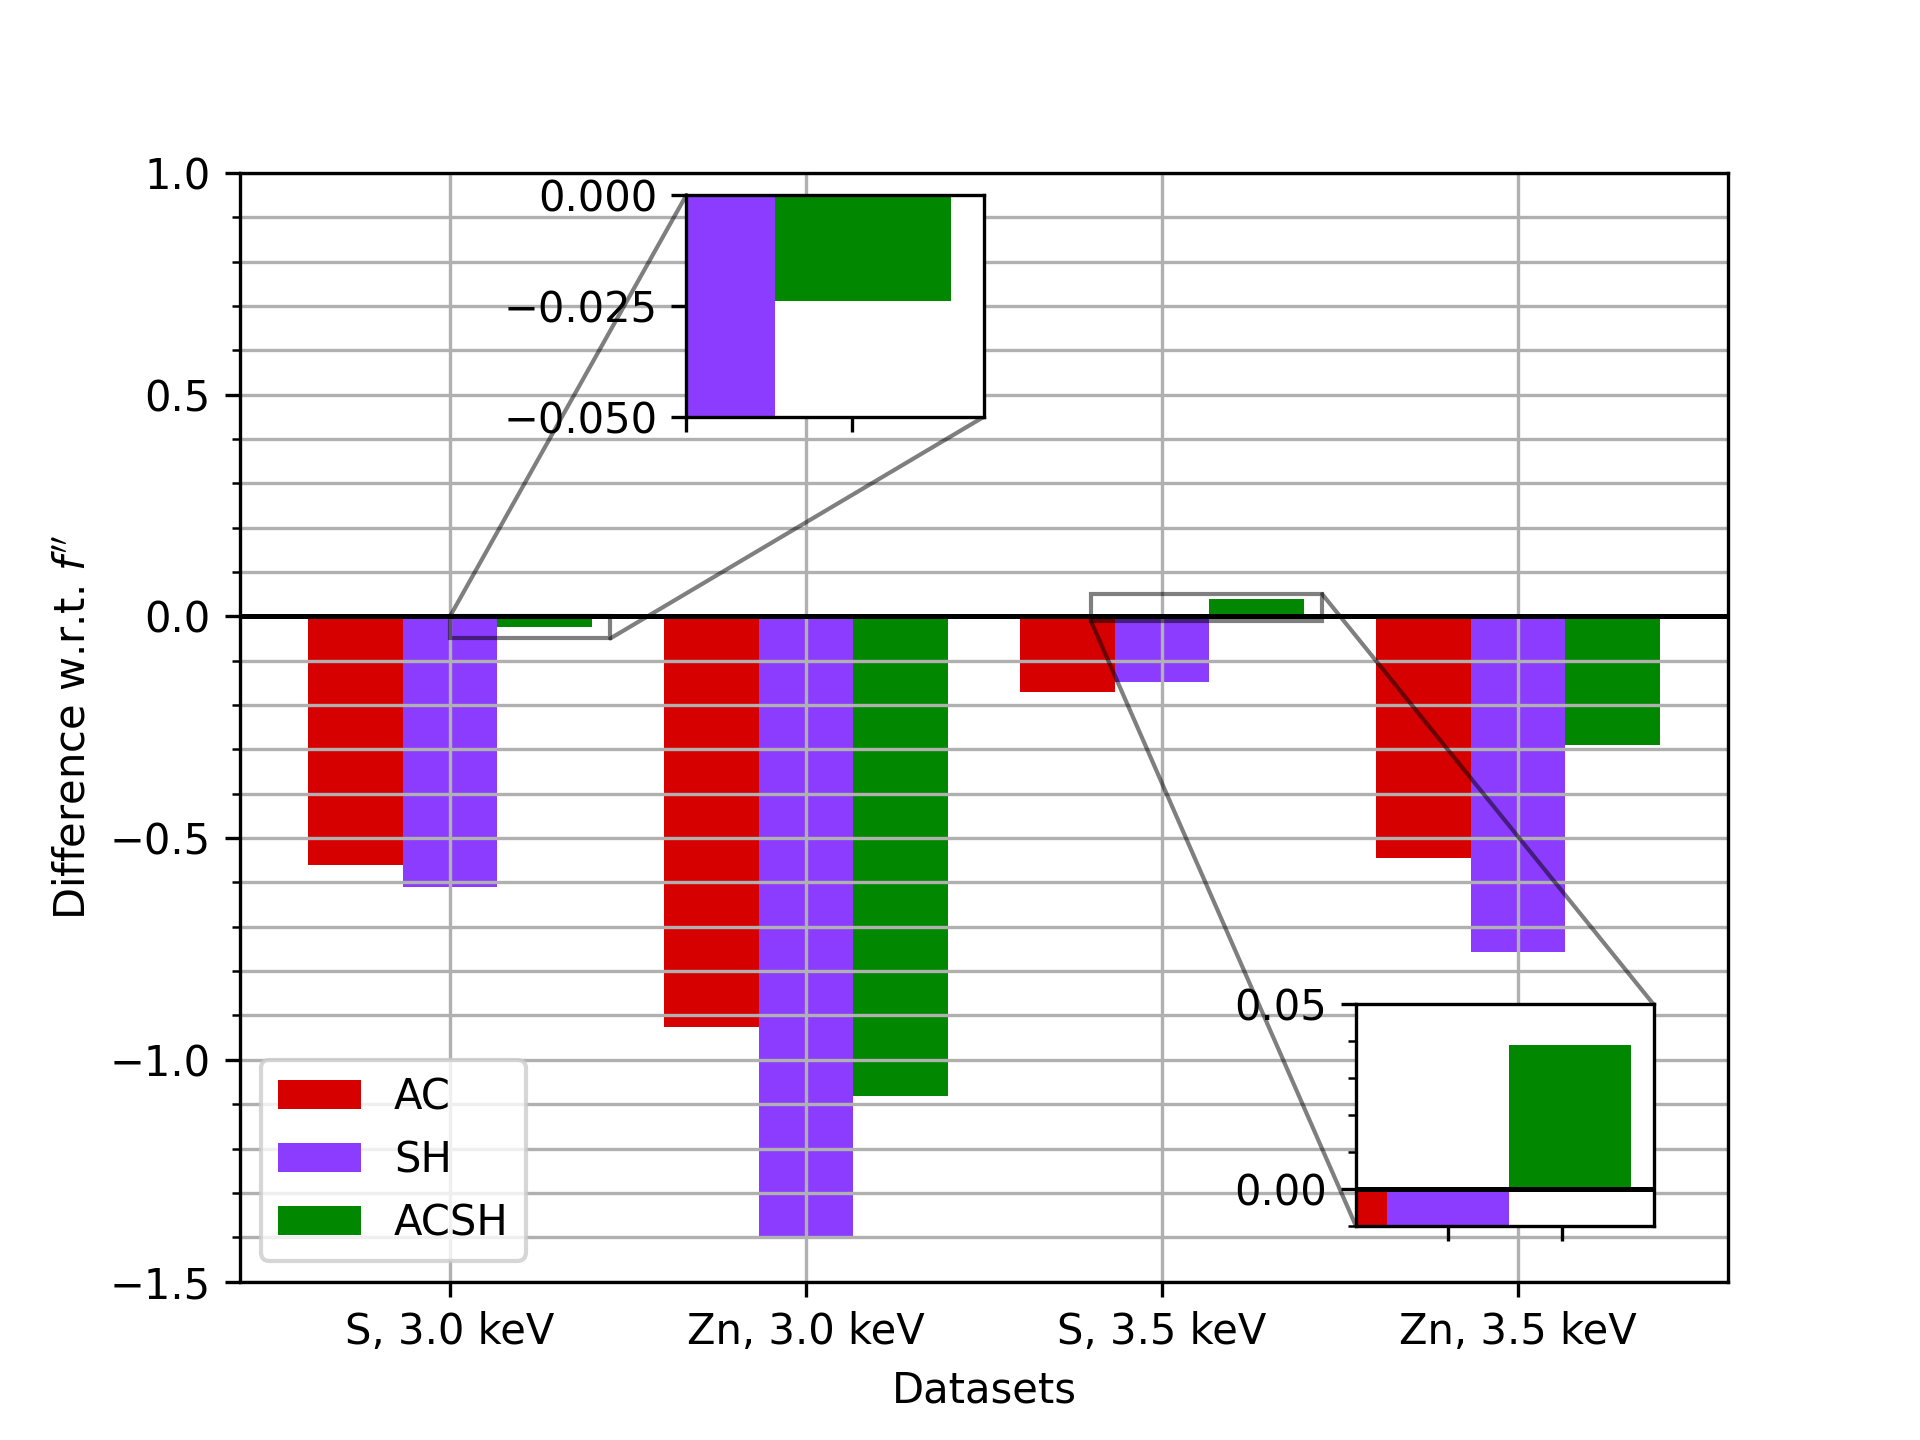
\includegraphics[width = 0.7\textwidth]{plots/phenix_plot_Pat.png}
    \caption{Difference with respect to theoretical $f"$ for atoms of sulphur and zinc in Thermolysin 2. Values obtained from Phenix.refine in the Phenix software package for Macromolecular structure determination.}
    \label{fig:phenix_plot}
\end{figure}

Results from Phenix refine for the six sets of reflection data of Thermolysin 2 (three methods across 3.0 and 3.5 keV) are shown in \cref{phenix_table} and visualized in \cref{fig:phenix_plot}. It is clear that refinement of the sulphur edge was much more precise than for zinc.


\subsection{Tomography-based corrections with laser-shaped samples}

\begin{figure}[h]
    \centering
    \begin{tabular}{cc}
    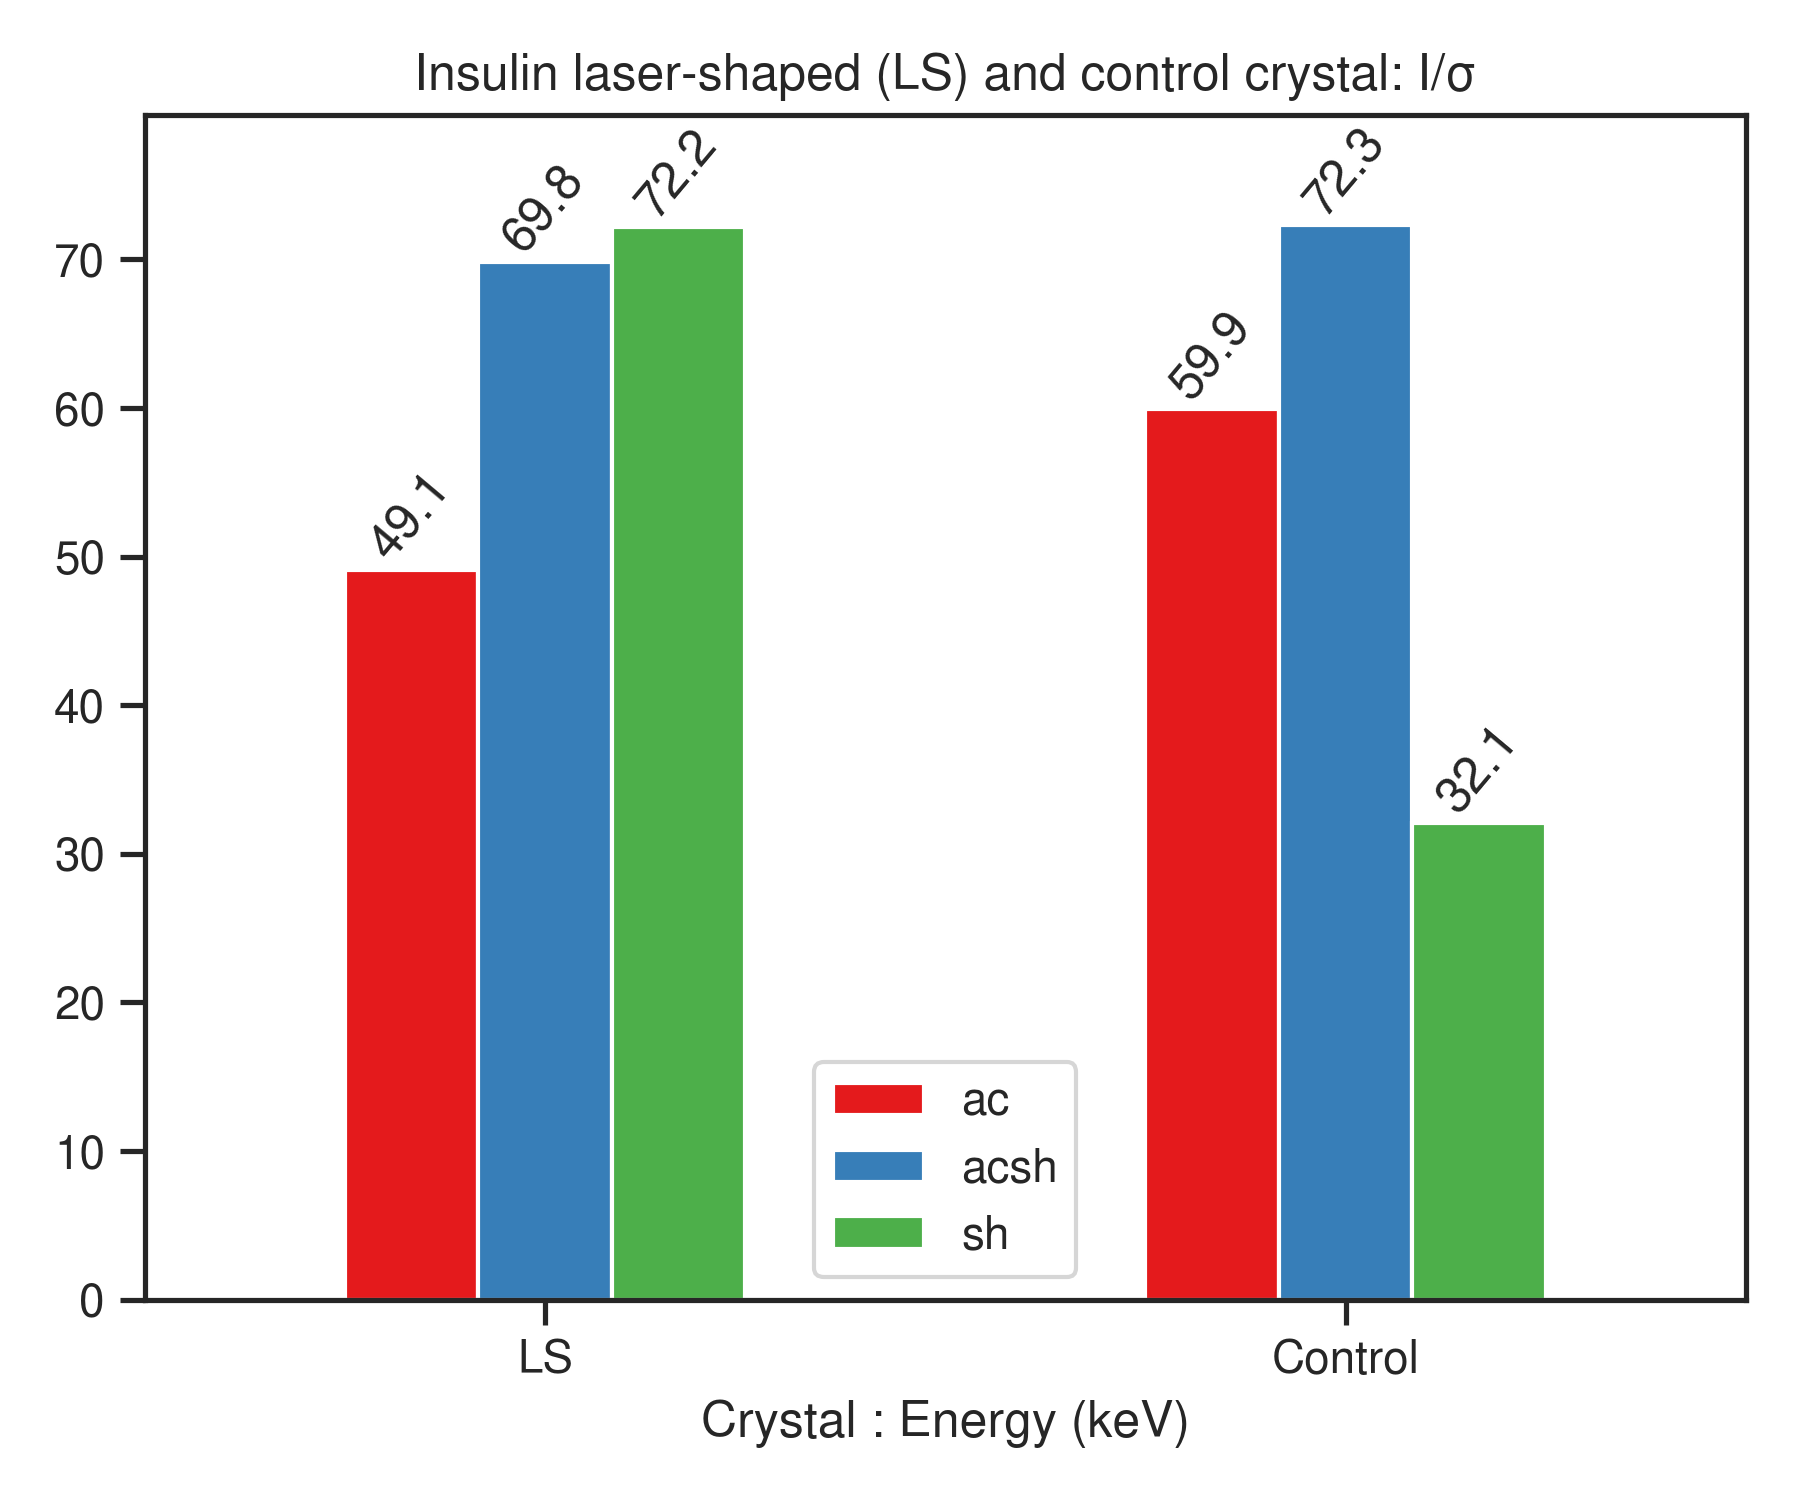
\includegraphics[width = 0.5\textwidth]{plots/exp2/ins_I_over_sigma.png} & 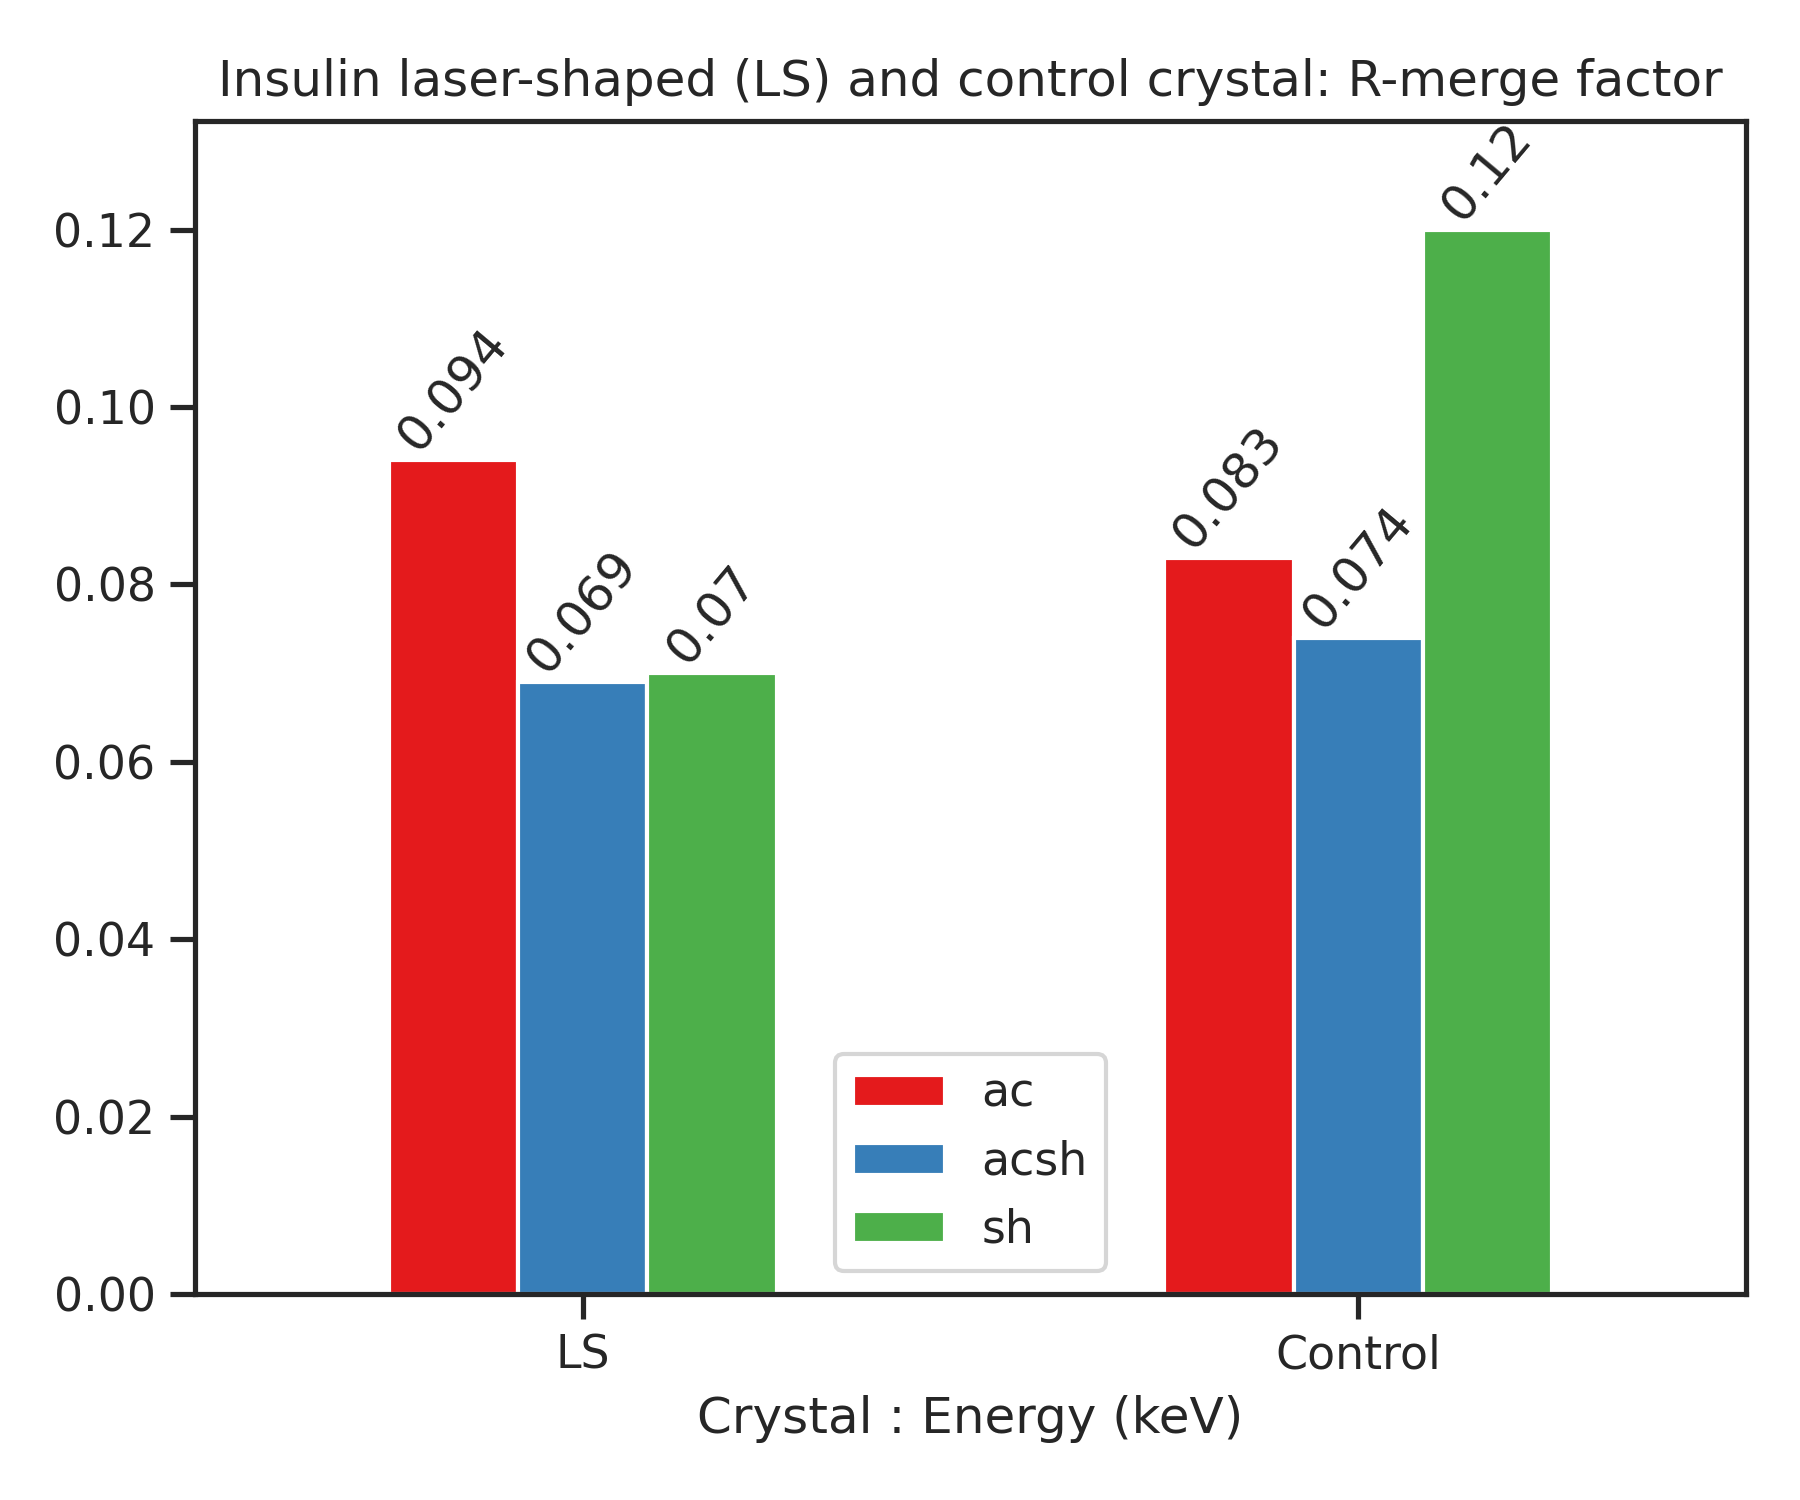
\includegraphics[width = 0.5\textwidth]{plots/exp2/ins_rmerges.png}
    \end{tabular}
    \caption{Merging statistics for the laser-shaped and control crystals of insulin at 3.0 keV.}
    \label{fig:insulin}
\end{figure}

\begin{figure}[h]
    \centering
    \begin{tabular}{cc}
    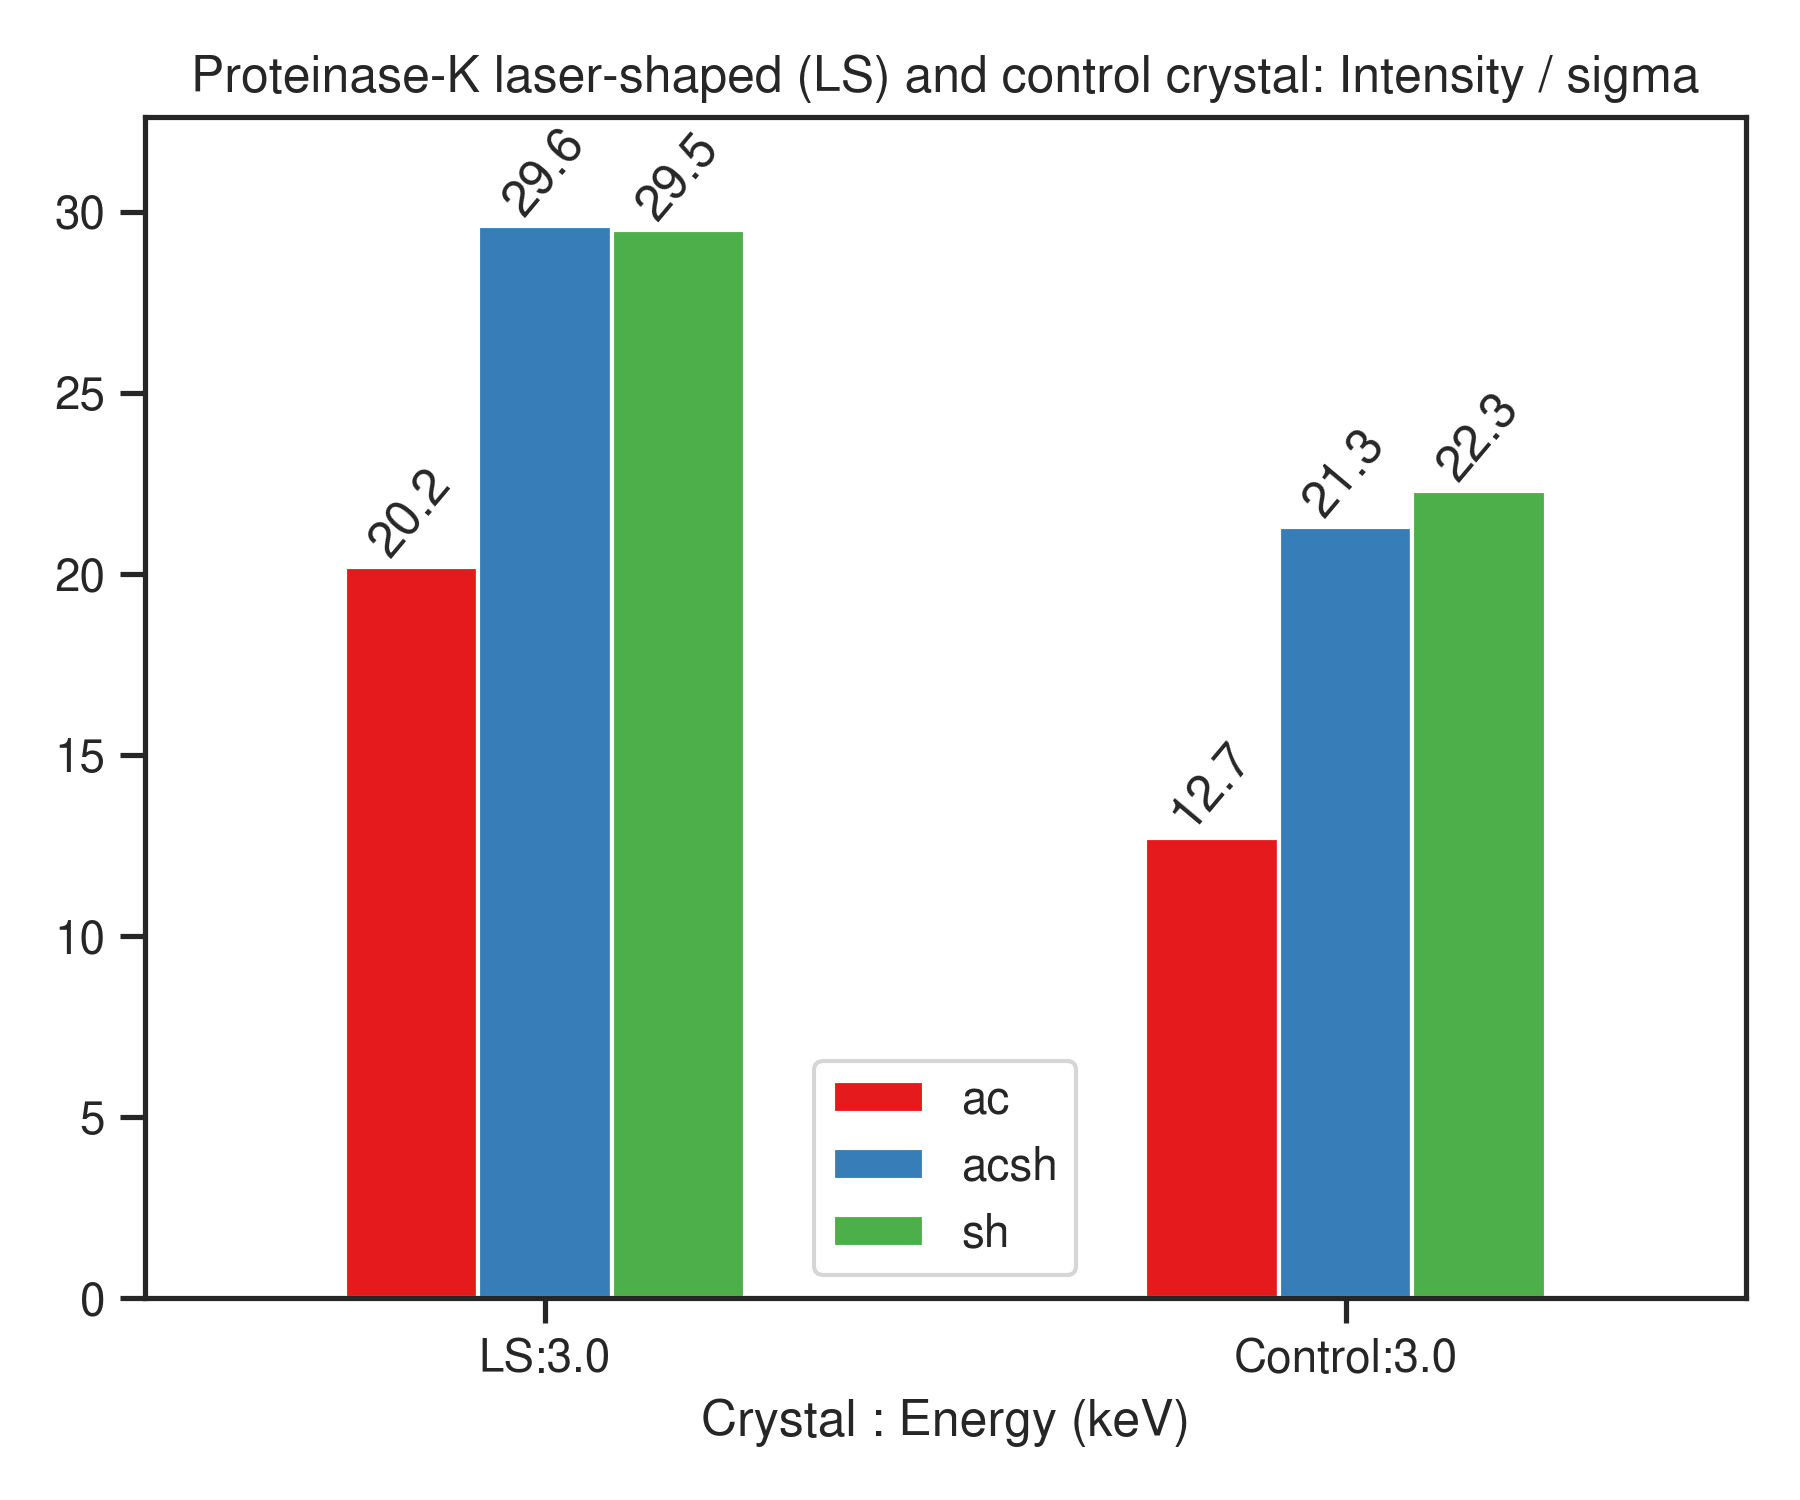
\includegraphics[width = 0.5\textwidth]{plots/exp2/prot_I_over_sigma.png} & 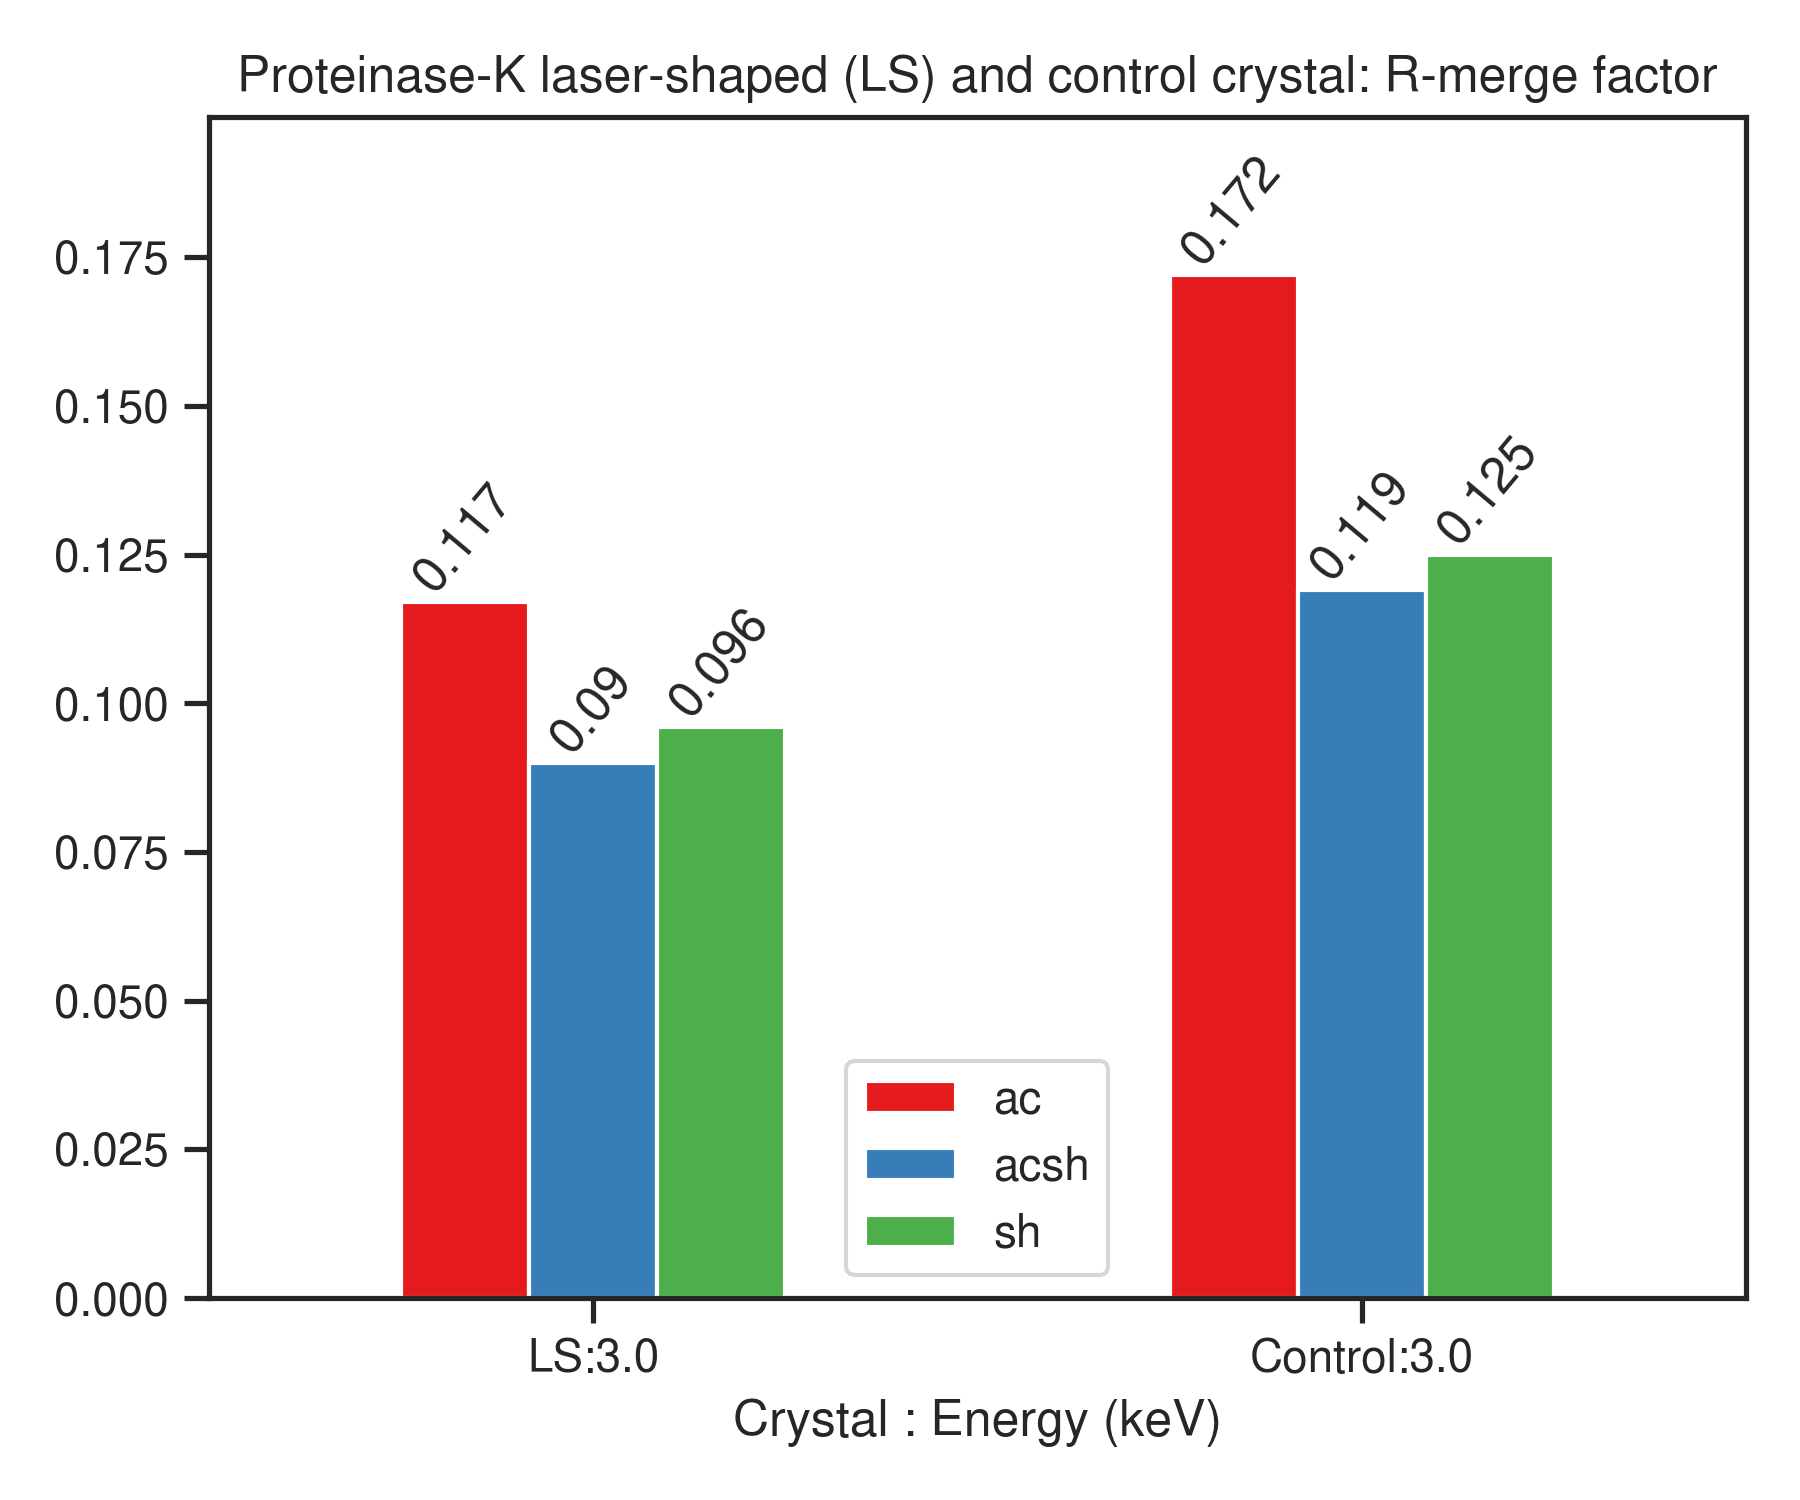
\includegraphics[width = 0.5\textwidth]{plots/exp2/prot_rmerges.png}
    \end{tabular}
    \caption{Merging statistics for the laser-shaped and control crystals of proteinasek at 3.0 keV.}
    \label{fig:proteinasek}
\end{figure}


Testing tomo on lysosyme to try to detect sodium anomalous signal

Mention LASER-shaping already worked on identifying magnesium in topoisomerase crystals. Hypothesis: tomography can do the same



\subsection{Errors and Improvement}

Faults in anacor thresholding, particularly at processing datasets collected at multiple energies

segmentation at high contrast

There are several challenges associated with the segmentation of X-ray data of protein crystals.